\documentclass[12pt]{My_preprint}
\title{
    %First moment of hydrodynamic forces on a translating spherical droplet immersed in a uniform flow at low but finite inertia effects.
    Rheology of a suspension made of non-buoyant spherical droplets
    }

\author[1,2]{Nicolas Fintzi and  Jean-Lou Pierson}

\normalmarginpar


\begin{document}

\maketitle

\begin{abstract}
    In this note, we use the reciprocal theorem to compute the first moment of hydrodynamic forces applied on a translating spherical droplet immersed in a uniform flow. 
    According to Hadamard-Rybczynski solution \citep{kim2013microhydrodynamics}, the first moment generated by the flow field surrounding a translating spherical droplet in a uniform flow, in the Stokes regime, is identically null. 
    In this study we consider finite but low droplet Reynolds number, $Re$, and compute the first order correction in $Re$ of the first moment of hydrodynamic forces. 
    It is shown that, in dimensionless form, the first moment is proportional to the square of the relative velocity times the Reynolds number.  
    The main consequence of that finding is that in a dilute emulsion of buoyant droplets, the effective stress is also proportional to the relative motion between phases and the Reynolds number. 
    % Particularly, we show that this stress have the form $\sim Re\phi [C_1\textbf{UU}+C_2\textbf{U}\cdot\textbf{U}]$ where $C_1$ and $C_2$ are constant of order one, and $\phi$ is the volume fraction. 
\end{abstract}


\section{Introduction}

Previous studies have shown how momentum exchange terms in multiphase flows equations, this includes the drag force, but also the first moment of forces (Stresslet and torque), and the second moment of forces, alter the rheological behaviors of the mixture.
\citet{einstein1905neue} and \citet{taylor1932viscosity} were the first to demonstrate how the symmetric part of the first moment of force (Stresslet) on solid sphere, and droplets, respectively, induces an additional viscosity to viscous dilute suspension. 
Then, years later \citet{lhuillier1996contribution,jackson1997locally,zhang1997momentum}, still considering viscous and dilute flows, demonstrated that the second moment of forces also contributes to the suspension Rheology, inducing non-Newtonian behaviors.
Because the second moment of forces appears under the divergence operator in the effective stress this term contributes to the ``non-homogeneous rheology''. 
Such rheological laws may also be referred to as second gradient fluids \citet{renee2023thermomecanique}.  

As identified in, \citet{fintzi2025averaged} the theoretical analysis regarding the computation of the effective stresses of suspensions are mainly limited to Stokes flows regime. 
Except for the studies of \citet{stone2001inertial} and later \citet{raja2010inertial}, which considered the effect of fluid inertia on neutrally buoyant, spheres and droplets, respectively, immersed in linear flows.
They computed the first moment of forces and the pseudo turbulent stresses in this configuration, accurate at $O(Re)$.  . 
In this case the mixture can be assimilated to a ``Reiner-Rivlin'' fluids, because it was found that the effective stress were proportional to the mean shear rate square (in the sateady-state regime). 

In this work we revisit the studies of~\citet{stone2001inertial,raja2010inertial}  to compute the Stresslet applied on a spherical droplet embedded in a uniform flow at low but finite inertia effects. 
In opposition to \citet{stone2001inertial} and \citet{raja2010inertial} who considered neutrally-buoyant sherical inclusion embedded in a shear flow, we focus on the relative motions of droplets with respect to the mixture velocity. 
Hence, our work differs in that we consider the effect of translation between the droplets and the ambient fluid on the effective stress of the suspension.
\citet{dabade2015} computed the torque (skew-symmetric part of the first moment) on a spheroidal particle embedded in a uniform flow. 
Hence, our study is similar to the work of \citet{dabade2015}, however we aim to compute the whole first moment tensor (not only the torque), and we consider droplets (instead of solid spheroidal particles). 

The originality of this work lies in the fact that we consider inertial buoyant droplets. 
Additionally, we compute the second moment of forces in addition to the Stresslet, thereby considering non-homogeneous rheological behaviors in the effective stress. 
The second key result of this study is the proposal of a general reciprocal relation that allows the computation of the second moment of forces on particles (not only of the drag force, and Stresslet). 
Finally, by following a rigorous statistical approach, we demonstrate how velocity variance terms appear in the ensemble-averaged expression of the interphase momentum exchange, and in the effective stress of the continuous phase. 
It must be said that we do not completely close the system of equations because we do not propose an explicit closure of the velocity variance terms that appear in the momentum equations. 



This manuscript is presented as follows: 
In~\ref{sec:context} we recall the averaged mass and momentum equations, and the closure terms to be computed. 
We show how the moments of forces are related to conditionally averaged quantities, which are governed by the equations presented in~\ref{sec:governing_equation}. 
To avoid the complete resolution of the equations, we derive in~\ref{sec:reciprocal} a general reciprocal relation that can be applied to derive the moments of forces of arbitrary order on droplets immersed in an arbitrary flows. 
This reciprocal relation also enables us to compute the internal shear rate (and related moments) of a droplet. 
Then, in~\ref{sec:compute_moments} we compute the $O(Re)$ of the moments of forces for droplets in pure translation with the ambient fluid. 
As a validation, in~\ref{sec:deformation} we show how to recover \citet{taylor1964deformation} from the Stresslet formula, and therefore demonstrate the direct link between effective stresses (Stresslet) and its counterpart, i.e., the deformation of droplets. 
Finally, in~\ref{sec:averaged_equations} we cast all the results into the averaged equations presented in~\ref{sec:context} and conclude on the rheological behaviors of the suspension. 

\section{Mathematical Context}\label{sec:context}


To better illustrate the role of various forces and stresses in a multiphase flow model, we begin by presenting the averaged mass and momentum equations for the dispersed and continuous phases, derived through an ensemble averaging procedure.
For mono-disperse emulsions, the mass and momentum equations of the continuous phase and dispersed phase can be written as \citep{fintzi2025averaged},
\begin{align}
    \label{eq:dt_phif}
    \phi_f + \phi &\approx 1,\\
    % \textbf{u}_f \phi_f + \textbf{u}_p \phi &\approx \textbf{u},\\
    \div \textbf{u} &= 0 
    \label{eq:div_u},\\
    \label{eq:dt_phip}
    % (\pddt + \textbf{u}_f  \cdot \grad) \phi_f
    % &= - \phi_f \div \textbf{u}_f,\\
    (\pddt + \textbf{u}_p \cdot \grad)\phi
    &=
    - \phi \div \textbf{u}_p,\\
    \label{eq:dt_up}
    \rho_p \phi  (\pddt + \textbf{u}_p \cdot \grad)\textbf{u}_p
    % + \div \pavg{m_p \textbf{u}_\alpha'\textbf{u}_\alpha'}
    &=
     \phi (\div \bm\Sigma
    + \rho_p  \textbf{g})
    + \div \bm\sigma_p^\text{eff}
    + \textbf{F}
    ,\\
    \rho_f \phi_f (\pddt + \textbf{u}_f  \cdot \grad) \textbf{u}_f
    &= \phi_f  \left(\div \bm{\Sigma}
    + \rho_f \textbf{g}\right)
    + \div \bm\sigma_f^{\text{eff}}
    - \textbf{F},
    \label{eq:dt_uf2}
\end{align}
respectively. 
The subscript $f$ and $p$ refer to continuous phase and droplets phase averaged quantities, respectively.
The vector $\textbf{g}$ is the acceleration of gravity and $\rho_k$ is the density of the phase $k$. 
We use the notation $\phi = n_p v_p$, with $n_p$ the droplets number density and $v_p$ the volume of a single droplet.
$\phi_f$ is the volume fraction of the continuous phase.
$\textbf{u}_f$ (resp. $\textbf{u}_p$) is the averaged velocity of the fluid (resp. dispersed) phase, $\bm\Sigma = - p_f \bm\delta + \mu_f [\grad \textbf{u} +  (\grad \textbf{u})^\dagger ]$ the \textit{mean Newtonian stress} of the mixture, with $p_f$ being the mean hydrodynamic pressure and $\textbf{u}=\phi_f \textbf{u}_f + \phi \textbf{u}_p$ the volume averaged velocity of the mixture.
$\bm{\sigma}^{\text{eff}}_p$ and $\bm{\sigma}^{\text{eff}}_f$ are the effective stresses of the dispersed and continuous phase, respectively.  
Finally, $\textbf{F}$ represents the interphase momentum exchange. 

The number density, continuous phase volume fraction, interphase force, and effective stresses of the dispersed and continuous phase, can be expressed formally as \citep{fintzi2025averaged},
\begin{align}
    n_p &= \pavg{}
    \label{eq:n_p},\\
    \phi_f &= \avg{\chi_f}
    \label{eq:chi_f},\\
    \textbf{F}  &= \pSavg{\bm\sigma^*_f\cdot \textbf{n}}
    \label{eq:f_alpha}
    ,\\
    \bm{\sigma}_p^{\text{eff}} &= -\pavg{\textbf{u}_\alpha'\textbf{u}_\alpha'}
    \label{eq:def_uup}
    ,\\
    \bm{\sigma}^{\text{eff}}_f 
    &= 
    - \avg{\chi_f\rho_f \textbf{u}_f'\textbf{u}_f'} 
    + \pavg{\intS{\textbf{r}\bm\sigma^{*}_f\cdot \textbf{n}} - \delta_p\intO{2\mu_f\textbf{e}_d^*}}\nonumber\\
    &- \div
        \pavg{ \frac{1}{2}\intS{\textbf{rr}\bm\sigma^{*}_f\cdot \textbf{n}}
        - \delta_p\intO{2\mu_f \textbf{r} \textbf{e}_d^*}}
        + \grad\grad (\ldots). 
    \label{eq:def_sigma_eff_f}
\end{align}
respectively. 
Where the operator $\avg{\ldots}$ corresponds to an ensemble average procedure,  $\chi_f$ is the phase indicator function of the continuous phase, $\delta_p = \sum_\alpha \delta(\textbf{x}-\textbf{x}_\alpha)$ the Dirac delta function pointing on the particle center of mass (denoted $\textbf{x}_\alpha$), and \textbf{n} the normal of the surface pointing outward the droplets. 
$\textbf{u}_\alpha$ is the center of mass velocity of a particle labeled $\alpha$. $\Omega_\alpha$ and $\Gamma_\alpha$, represent the domains of the volume and surfaces, of the droplets $\alpha$, respectively. 
The superscript $'$ indicates the relative values of a quantity with respect to its phase-averaged value. 
Specifically $p_f' = p_f^0 - p_f$, $\textbf{u}_\alpha' = \textbf{u}_\alpha - \textbf{u}_p$ and $\textbf{u}_f' = \textbf{u}_f^0  -\textbf{u}_f$, with $\textbf{u}_f^0$ and $p_f^0$,  the local velocity and pressure fields of the continuous phase, respectively. 
The superscript $^*$ represents the relative values of a quantity with respect to the mixture volume averaged value, such that $\bm{\sigma}_f^* = \bm{\sigma}_f^0  - \bm{\Sigma}$ and $\textbf{e}_d^* = \textbf{e}_d^0 - \textbf{E}$, where $\bm{\sigma}_f^0 = -p_f^0 + \mu_f [\grad \textbf{u}_f^0 + (\grad \textbf{u}_f^0)^\dagger]$ is the local stress of the continuous phase, and $\textbf{e}_d^0 =\frac{1}{2}(\grad \textbf{u}_d^0+^\dagger\grad \textbf{u}_d^0)$, is the internal shear rate within the droplet phase.
Note that, $\textbf{u}_d^0$ is the internal velocity of the fluid within the droplets, in opposition to $\textbf{u}_p$ which is the average of the center of mass velocity. 




In the present situation the ``closure problem'' consists in finding explicit expressions for the terms of the form $\avg{\ldots}$, in \ref{eq:f_alpha}, \ref{eq:def_uup} and \ref{{eq:def_sigma_eff_f}}, in terms of the unknown of the problem, i.e. $n_p$, $\phi_f$, $p_f$, $\textbf{u}_p$ and $\textbf{u}_f$. 
In this work we focus on the last two terms of $\bm\sigma^\text{eff}_f$, i.e. the first and second moment of hydrodynamic forces acted upon spherical droplets.
Hence, the closure problem is to find an expression for the disturbance fields $\bm\sigma_f^*$ and $\textbf{e}_d^*$. 
Because they are evaluated at the surface and in the interior of the test droplets, these terms may be written as, 
\begin{align}
    \bm\sigma_f^* =p_f' \bm\delta 
    + \mu_f [\grad \textbf{u}^* + (\grad \textbf{u}^*)^\dagger]
    && 
    \textbf{e}_d^* = [\grad \textbf{u}^* + (\grad \textbf{u}^*)^\dagger] /2
    \label{eq:conditional_average}
\end{align}
with $\textbf{u}^* = \textbf{u}^0 - \textbf{u}$ and $\textbf{u}^0$ the local velocity of the mixture\footnote{
    This is because $\delta_p \textbf{u}^0_f=\delta_p  \textbf{u}^0$ at the surface of the test droplet, and $\delta_p \textbf{u}_d^0 = \delta_p \textbf{u}^0$ in its interior.
    Indeed, the test droplet is fixed on every configuration due to the presence of the distribution $\delta_p$. 
}. 

Because the emulsion is assumed mono-disped and the droplets are assumed spherical, the surface exchange terms may be re-written in terms of integrals of conditional averaged quantities \citep{lhuillier1992ensemble,zhang1997momentum,fintzi2025}. 
If we take the example of the drag force term, using~\ref{eq:conditional_average}, we obtain, 
\begin{equation}
    \pSavg{\bm\sigma^*_f\cdot \textbf{n}}
    =
    \int_{\mathbb{R}^3} P[\textbf{w}|\textbf{x},t] n_p[\textbf{x},t]\intS[p]{
        \left\{
            p_f^1 \bm\delta 
    + \mu_f [\grad \textbf{u}^1 + (\grad \textbf{u}^1)^\dagger]
        \right\}\cdot \textbf{n}
    }(\textbf{r})  
    d^3 \textbf{w},
    \label{eq:conditional_average2}
\end{equation}
where $p_f^1[\textbf{r}|\textbf{x},\textbf{w}]$ and $\textbf{u}^1[\textbf{r}|\textbf{x},\textbf{w}]$, are the pressure and velocity field ensemble averaged on every configuration where a particle is located at $\textbf{x}$ with center of mass velocity \textbf{w}, minus the (unconditionally) ensemble averaged  pressure and velocity fields (i.e. $p_f[\textbf{r},t]$, and $\textbf{u}[\textbf{r},t]$).
Here, $ P[\textbf{w}|\textbf{x},t]$ is the probability of finding a droplet with center of mass velocity \textbf{w} knowing that the droplet is present at \textbf{x} at time $t$. 
As it will be presented in the next section, the equations governing these fields can be obtained by conditionally averaging the local mass and momentum equations.
% In our context of approximation (accurate at $O(\phi)$, $O(Re)$) this leads to Maxey-Riley-Gatignol equations around a test droplet \citep{fintzi2025}. 
So that the boundary conditions of the conditional problem are well-defined, one must average only on configurations which posses similar boundary condition at the surface of the test droplet. 
Hence, conditionally averaging on the position \textbf{x}, and center of mass velocity \textbf{w} is a necessary step in the procedure\footnote{
    Note that we used conditional average in terms of center of mass velocity, this is because we seek an expression of the force in terms of the center of mass velocity $\textbf{w}$. 
    If we were looking for add mass terms, it would be required to conditionally average~\ref{eq:conditional_average2} by the center of mass acceleration of the droplet, for example. 
    Likewise, for non-spherical particles it is necessary to conditionally average the local fields ($p_f^1$ and  $\textbf{u}^1$) by the instantaneous shape of the particle, and then integrate overall probable geometry \citep{lhuillier1992ensemble}. 
}.

In the following we consider arbitrary values of density and viscosity ratios: 
\begin{align}
    \lambda = \mu_p/\mu_f,  && \zeta =\rho_p /\rho_f,
\end{align}
where $\mu_p$ and $\rho_p$ are the viscosity and density of the droplets, respectively.
Additionally, we limit this theoretical investigation to dilute suspensions ($\phi\ll 1$), and we consider small but finite values of the droplet Reynolds number, defined as,
\begin{equation}
    Re  = \frac{U\rho_f a}{\mu_f}, 
\end{equation}
where $a$ is the radius of the droplets, and $U = |\textbf{u} - \textbf{w}|$ the magnitude of the relative velocity between the center of mass velocity of the test droplet, and the ensemble averaged velocity of the mixture. 
Note that the velocity scale, $a |\grad \textbf{u}|$, and $a^2 |\grad\grad \textbf{u}|$ may be different from the relative uniform velocity scale: $|\textbf{u} - \textbf{w}|$. 
Nevertheless, although linear and quadratic flow may be present, only inertial effects due to relative uniform motions are considered, therefore we consider that: $0 < a |\grad \textbf{u}|\approx a^2 |\grad\grad \textbf{u}| \ll U$. 
Finally, the \textit{capillary} number,
\begin{equation}
    Ca = \mu_f U/\gamma,
\end{equation}
is assumed to be so small that the droplets remain spherical. 


The values of $\bm\sigma_f^*$ and $\textbf{e}_d^*$ will only be accurate at order $O(1)$ in $\phi$ (neglecting the droplets interactions), and $O(Re)$ in the Reynolds number based on~$U$. 
Hence, after integration over the surface of the droplet, and all velocities $\textbf{w}$ (see~\ref{eq:conditional_average2}), the force, first moment of force and second moment, will add a contribution of $O(Re \phi)$ in the averaged momentum equations~\eqref{eq:dt_uf2}. 



% \section{The reciprocal theorem and equaitons for a droplet force and Stresslet}
% \label{ap:reciprocal}




\section{Governing equations and solutions}


At the leading order in droplet volume fraction, the governing equations for $\textbf{u}^*$ and $p_f'$ is equivalent to that of an isolated droplet in an infinite medium \citet{hinch1977averaged}. 
Hence, we consider the problem of an isolated test droplet immersed in an arbitrary flow. 
The disturbances pressure and velocity field relative to the position of a test droplet are noted $\textbf{u}_{o}$, $\textbf{u}_{i}$, $p_{o}$ and $p_{i}$, for the velocity outside the test droplet, the velocity inside the droplet, the pressure outside the droplet and the pressure inside the droplet, respectively. 
In the following the center of mass velocity of the droplet is noted $\textbf{w}$. 
Note that because $\textbf{u}_o$ and $p_o$ are defined as a disturbance fields they vanish far from the position of the test droplets. 
On~\ref{fig:disturbance} we display a schematic representation of the problem. 
\begin{figure}[h!]
    \centering
    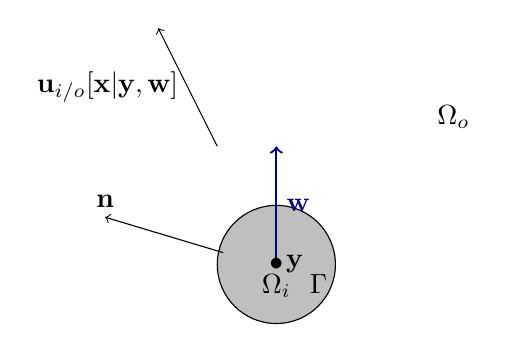
\begin{tikzpicture}[scale= 1.5]
        \filldraw[ gray!50!white](0,0)circle (0.5);
        \draw(0,0)circle (0.5)node[right,below]{   $\;\;\;\;\;\;\;\;\;\;\;\Gamma$};
        \draw[->,blue!50!black,thick](0,0)--++(0,1)node[midway,right]{$\textbf{w}$};
        \draw (0,0)node{$\bullet$}node[right]{$\textbf{y}$};
        \draw[->] (-0.45,0.1)--++(-1,0.3)node[above]{$\textbf{n}$};
        \draw[->](-0.5,1)--++(-0.5,1)node[midway,left]{$\textbf{u}_{i/o}[\textbf{x}|\textbf{y},\textbf{w}]$};
        % \draw[->] (3,1)node{$\bullet$}--++(0,1.5)node[right,midway]{$\textbf{u}_f[\textbf{x}]$};
        \draw (0,0)node[below]{$\Omega_i$};
        \draw (1.5,1.25)node{$\Omega_o$};
    \end{tikzpicture} 
    \caption{Representation of the problem parameters. $\textbf{u}_{o/i}[\textbf{x},\textbf{y}]$ is the disturbance velocity field evaluated at \textbf{x}, generated by a test droplet positioned at \textbf{y}. \textbf{n} is the unit normal  pointing outward the droplet, and \textbf{w} the droplet center of mass velocity. 
    The domain of the exterior of the droplet is noted $\Omega_o$ and the one the interior $\Omega_i$.}
    \label{fig:disturbance}
\end{figure}

\subsection{Maxey, Riley \& Gatignol's equations}

Outside and inside the volume of the test droplet we can write the mass and momentum equations for the disturbances fields $p_{o/i}$ and $\textbf{u}_{o/i}$ by conditionally averaging the navier stokes equations \citet{fintzi2025}, or simplify by considering the equations derived by \cite{maxey1983equation} \& \citet{gatignol1983faxen}. 
It reads, 
\begin{align}
    \div \textbf{u}_{o} &= 0
    \\
    \div\bm\sigma_{o}
    &= 
    Re [
    \pddt \textbf{u}_{o}
    + \textbf{u}_{o}\cdot \grad \textbf{u}_{o}
    + \textbf{u}_{o}\cdot \grad \textbf{u}_r
    + \textbf{u}_r \cdot \grad \textbf{u}_{o}]
    = Re \textbf{f}_{o}
    \label{eq:momentum_out}
\end{align}
and, 
\begin{align}
    \div \textbf{u}_{i} &= 0,
    \\
    \div\bm\sigma_{i}
    &= 
    \frac{\zeta}{\lambda}Re [
    \pddt \textbf{u}_{i}
    + \textbf{u}_{i}\cdot \grad \textbf{u}_{i}
    + \textbf{u}_{i}\cdot \grad \textbf{u}_r 
    + \textbf{u}_r \cdot \grad \textbf{u}_{i}]
    = \frac{\zeta}{\lambda}Re \textbf{f}_{i}
    \label{eq:momentum_in}
\end{align}
\tb{introduce the dimensionless number (but $\textbf{u}_r$ is acctually unit vect herre)}
where we introduced the relative velocity $\textbf{u}_r = \textbf{u} - \textbf{w}$.  
We recall here that \textbf{u} is the undisturbed, or ensemble averaged velocity, present in~\ref{eq:dt_uf2}.
Additionally, $\bm\sigma_{i/o} = -p_{i/o}\bm\delta + 2\textbf{e}_{i/o}$ with $\textbf{e}_{i/o} = \frac{1}{2}[\grad \textbf{u}_{i/o} + ^{\dagger}\grad \textbf{u}_{i/o}]$ is the dimensionless newtonian stresses of each phase. 
% We introduce the Reynolds number $Re = \frac{\rho_f a |\textbf{u}_r|}{\mu_f}$ based on the droplet radius $a$, the density ratio $\zeta = \rho_d / \rho_f$ and the viscosity ratio $\lambda = \mu_d / \mu_f$. 
Note that the distances have been made dimensionless using $a$, and the velocities by $|\textbf{u}_r|$ in the above equation. 

At the surface of the droplet ($r = 1$) the continuity of velocity and the non-deformability of the test droplet imposes, 
\begin{align}
    \textbf{u}_{i} = \textbf{u}_{o}
    && 
    \textbf{u}_{i} \cdot \textbf{n}
    =
    - \textbf{u}_r \cdot \textbf{n}
    \label{eq:normal_vel}
\end{align}
where it must be noted that both $\textbf{u}_{i}$ and $\textbf{u}$ are evaluated at the points on the surface of the droplet, hence $\textbf{u}_r$ may not always be a constant vector. 
The undisturbed or ensemble averaged shear rate of the continuous phase reads  $\textbf{E} =\frac{1}{2} [\grad \textbf{u} + ^\dagger \grad \textbf{u}]$. 
Note that for instance the ensemble averaged quantities $\textbf{u}$ and $\textbf{E}$ are kept general, hence their values depends on the position along the surface of the test droplet. 
At the interface of the test droplet the tangential shear rate is assumed continuous, however because it is the total shear rate field (and not just $\textbf{e}_{i/o}$) that satisfy this condition, we obtain (at $r=1$),
\begin{equation}
    \mathbf{n}\cdot [\textbf{e}_{o} - \lambda \textbf{e}_{i} + (1-\lambda)\textbf{E}
    % - \textbf{b}
    ]\cdot (\bm\delta - \textbf{nn})
    =
    \textbf{b}\cdot (\bm\delta - \textbf{nn})
    % 0
    \label{eq:boundary_cdt_stress}
\end{equation}
with, 
\begin{equation}
    \textbf{b}
    =
    \frac{a \grad \gamma}{2 \mu_f |\textbf{u}_r|}
    = Ma \grad\gamma /|\grad \gamma|. 
\end{equation}
Where we have considered Marangoni stresses, with $Ma = \frac{a |\grad \gamma|}{2 \mu_f |\textbf{u}_r|}$. 



% where we have introduced the relative velocity field $\textbf{U}[\textbf{x},t] = \textbf{w} - \textbf{U}_f[\textbf{x},t]$. 
Far from the test droplet it is assumed that the disturbance fields are vanishingly small hence the final requirement on $p_{o}$ and $\textbf{u}_{o}$ are, 
\begin{align*}
    \lim_{|\textbf{x}-\textbf{y}|\to\infty }\textbf{u}_{o}[\textbf{x}|\textbf{y}] = 0,
    && \lim_{|\textbf{x}-\textbf{y}|\to\infty }p_{o}[\textbf{x}|\textbf{y}]= 0. 
\end{align*}
We recall that $\textbf{y}$ is the position of the test droplet and \textbf{x} a point of evaluation. 





\subsection{Stokes flow solution for a droplet embedded in a quadratic flow}
The Reciprocal theorem requires the use of a known solution.
We call that solution the \textit{test} solution, since its only purpose is to compute the \textit{real} solution of the equations introduced above. 
We note the \textit{test} velocity and stress fields $\hat{\textbf{u}}_{i/o}$ and $\hat{\bm\sigma}_{i/o} = - \hat{p}_{i/o}\bm\delta + \grad \hat{\textbf{u}}_{i/o} + ^\dagger\grad \hat{\textbf{u}}_{i/o}$, respectively. 

In this problem we neglect all inertial effects and consider an arbitrary quadratic flow. 
In this situation $\hat{p}_{out/in}$ and $\hat{\textbf{u}}_{out/in}$ satisfy,
\begin{align}
    \div \hat{\textbf{u}}_{o} = 0 
    &&\div\hat{\bm\sigma}_{o}  = 0 
    \label{eq:momentum_out_s}\\
    \div \hat{\textbf{u}}_{i} = 0 
    && \div\hat{\bm\sigma}_{i}  = 0 
    \label{eq:momentum_in_s}
\end{align}
with the boundary conditions, 
\begin{equation}
    \lim_{|\textbf{x}-\textbf{y}|\to \infty}(\hat{\textbf{u}}_{o},p_{o}) = (\textbf{0},0) 
\end{equation}
and (at $r=1$),
\begin{align}
    \hat{\textbf{u}}_{i} &= \hat{\textbf{u}}_{o}\\
    \hat{\textbf{u}}_{i} \cdot \textbf{n} &= - \hat{\textbf{u}}_r \cdot \textbf{n}
    \label{eq:normal_vel_s}
    \\
    \mathbf{n}\cdot [\hat{\textbf{e}}_{o} - \lambda \hat{\textbf{e}}_{i} + (1-\lambda) \hat{\textbf{E}}
    % - \hat{\textbf{b}}
    ]\cdot (\bm\delta - \textbf{nn})
    &=
    \hat{\textbf{b}}\cdot (\bm\delta - \textbf{nn})
    % 0
\end{align}
where we introduced $\hat{\textbf{u}}_r = \hat{\textbf{u}} - \textbf{w}$ as the ensemble or undisturbed velocity field of the test problem, similarly $\hat{\textbf{E}}$ is the undisturbed stress of the test problem. 


For our purposes we only need $\hat{\textbf{b}}$ and $\hat{\textbf{u}}$ to be quadratic fields.
Hence, we introduce the relations, 
\begin{align*}
    \hat{\textbf{u}}(\textbf{y} + \textbf{n}) 
    &=  \hat{\textbf{u}}_r|_{\textbf{r}=0}
    +  \textbf{r} \cdot  \grad\hat{\textbf{u}}|_{\textbf{r}=0}
    +  \frac{1}{2}\textbf{rr} :  \grad\grad\hat{\textbf{u}}|_{\textbf{r}=0}
    + \ldots\\
     \hat{\textbf{E}}(\textbf{y} + \textbf{n}) 
    &=   \hat{\textbf{E}}|_{\textbf{r}=0}
    + \textbf{r} \cdot  \grad \hat{\textbf{E}}|_{\textbf{r}=0}
    + \frac{1}{2}\textbf{rr} :  \grad\grad \hat{\textbf{E}}|_{\textbf{r}=0}
    + \ldots\\
     \hat{\textbf{b}}(\textbf{y} + \textbf{n}) 
    &=   \hat{\textbf{b}}|_{\textbf{r}=0}
    + \textbf{r} \cdot  \grad \hat{\textbf{b}}|_{\textbf{r}=0}
    + \frac{1}{2}\textbf{rr} :  \grad\grad \hat{\textbf{b}}|_{\textbf{r}=0}
    + \ldots
\end{align*}
According to the linearity of the Stokes equations we deduce that $\textbf{u}_{i/o}$ and $p_{i/o}$  must be linear combination of spherical harmonics proportional to $\textbf{u}|_{\textbf{x}=0}$, $\grad \gamma|_{\textbf{x}=0}$, and their derivatives \citep{brenner1963resistance}.
Hence, we can write that the disturbance velocity and pressure fields are given by, 
\begin{align}
    \begin{pmatrix}
        \hat{\textbf{u}}_{o}\\
        \hat{p}_{o}\\
        \hat{\textbf{u}}_{i}\\
        \hat{p}_{i}
    \end{pmatrix}
    =
    \begin{pmatrix}
        \textbf{U}_{o}^{(1)} + \textbf{U}_{o}^{(2)}\cdot \grad + \textbf{U}_{o}^{(3)} :\grad\grad &
        \textbf{U}_{o}^\text{(b-1)} + \textbf{U}_{o}^\text{(b-2)}\cdot \grad + \textbf{U}_{o}^\text{(b-3)} :\grad\grad \\
        \textbf{P}_{o}^{(1)} + \textbf{P}_{o}^{(2)}\cdot \grad + \textbf{P}_{o}^{(3)} :\grad\grad &
        \textbf{P}_{o}^\text{(b-1)} + \textbf{P}_{o}^\text{(b-2)}\cdot \grad + \textbf{P}_{o}^\text{(b-3)} :\grad\grad \\
        \textbf{U}_{i}^{(1)} + \textbf{U}_{i}^{(2)}\cdot \grad + \textbf{U}_{i}^{(3)} :\grad\grad &
        \textbf{U}_{i}^\text{(b-1)} + \textbf{U}_{i}^\text{(b-2)}\cdot \grad + \textbf{U}_{i}^\text{(b-3)} :\grad\grad \\
        \textbf{P}_{i}^{(1)} + \textbf{P}_{i}^{(2)}\cdot \grad + \textbf{P}_{i}^{(3)} :\grad\grad &
        \textbf{P}_{i}^\text{(b-1)} + \textbf{P}_{i}^\text{(b-2)}\cdot \grad + \textbf{P}_{i}^\text{(b-3)} :\grad\grad \\
    \end{pmatrix}
    \cdot 
    \begin{pmatrix}
        \hat{\textbf{u}}_r\\
        \hat{\textbf{b}}
    \end{pmatrix}
    \label{eq:big_solution}
\end{align}
The tensor $\textbf{U}_{i/o}^{(n)}$ and $\textbf{P}_{i/o}^{(n)}$ are $n+1$ and $n$ order tensors given in \citet[Appendix F]{fintzi2024averaged}, that depend only on the coordinate $\textbf{r} = \textbf{x}-\textbf{y}$ and the viscosity ratio $\lambda$.
We also define the $n+2$ order tensors\footnote{The $^\dagger$ is used to indicate the transpose operator which acts on the two closet index, example the triadic $^\dagger\textbf{abc} = \textbf{bac}$ while $\textbf{abc}^\dagger = \textbf{acb}$. }, 
\begin{equation}
    \textbf{S}_{i/o}^{(n)} = 
    - \bm\delta\textbf{P}_{i/o}^{(n)}
    + \grad \textbf{U}_{i/o}^{(n)}
    + ^\dagger\grad \textbf{U}_{i/o}^{(n)},
    \label{eq:big_S}
\end{equation}
which provide the stresses fields upon contraction with $\textbf{u}_r$, $\textbf{b}$, and the higher derivatives. 

\subsection{Point source solution}



Following \citet{stone2001inertial} we also consider the test problem of a point source of strength $Q$ located at the center of the sphere (\textbf{y}).
In this case the test velocity  and stress fields, reads\citep{pozrikidis2011introduction,pozrikidis1992boundary}, 
\begin{align}
    \hat{\textbf{u}}_{o/i} = \frac{Q}{4\pi} \textbf{n}r^{-2}
    && \hat{\bm\sigma}_{o/i} = \mu_f \frac{Q}{2\pi}\left(
        \bm\delta
        - 3 \textbf{nn}
    \right)r^{-3}
    \label{eq:point_source}
\end{align}
Note that this expression is valid throughout the domain excluding the point $\textbf{r} =  \textbf{x} -  \textbf{y} = 0$, hence we may use either the subscript $o$ or $i$. 
The reason why this solution is necessary is because, in the previous test problem $\div \hat{\textbf{u}}= 0$ (in opposition to what we have in~\ref{eq:point_source}), hence the previous solution was unable to provide a formula for the trace of the first moment using the reciprocal theorem \citep{stone2001inertial}.

In summary, as the values of $\hat{\textbf{u}}_r$, $\hat{\textbf{b}}$ and $Q$ are entirely arbitrary, the solutions given by~\ref{eq:big_solution} and~\ref{eq:point_source} will be used as a tool to derive formula for the drag forces, first moment, and second moment of hydrodynamic forces, using the reciprocal theorem derived in the next section.  

\section{Reciprocal theorem for droplets}

% We now demonstrate how to derive the reciprocal theorem for droplets.
A similar derivation to what is presented here may be found in \citet{lovalenti1993force,raja2010inertial}, however we hope to provide some clarifications and generalization, by exposing a detailed and simpler demonstration.  

The derivation of the general formula goes into three steps: (1) we write the reciprocal theorem in the exterior of the droplet, (2) then on the interior of the droplet, (3) then using the boundary condition at the interface of the droplet we write the final formula. 

\subsection{First step:}
We first take the dot product of~\ref{eq:momentum_out} with $\hat{\textbf{u}}_{o}$, and the dot product of~\ref{eq:momentum_out_s} with $\textbf{u}_{o}$, subtracting both expression gives, 
\begin{equation}
    \div (\bm\sigma_{o}\cdot \hat{\textbf{u}}_o)
    % - \bm\sigma_o :\grad \hat{\textbf{u}}_o
    % \hat{\textbf{u}}_{o} \cdot (\div \bm\sigma_{o})
    =
    \div (\hat{\bm\sigma}_{o}\cdot \textbf{u}_o)
    % - \hat{\bm\sigma}_o :\grad \textbf{u}_o
    + Re (\hat{\textbf{u}}_{o}\cdot \textbf{f}_{o}). 
    \label{eq:first_step_out}
\end{equation}
To derive this relation we used the fact that $\bm\sigma_o :\grad \hat{\textbf{u}}_o = 2\textbf{e}_o :\grad \hat{\textbf{u}}_o = 2{\textbf e}_o : \hat{\textbf e}_o$, and  $\hat{\bm\sigma}_o :\grad {\textbf{u}}_o = 2\hat{\textbf{e}}_o : \textbf{e}_o$, leading to $\bm\sigma_o :\grad \hat{\textbf{u}}_o = \hat{\bm\sigma}_o :\grad {\textbf{u}}_o$. 
This simplification is the reason why the complete knowledge of the velocity field becomes unnecessary with the reciprocal theorem when $\textbf{f}_o = 0$.
Consequently, the  efficiency of the reciprocal theorem is rooted in the commutativity of the operation $\textbf e_o:\hat{\textbf e}_o$. 
Integrating this expression on the whole domain $\Omega_{o}$, and injecting the relations $\textbf{u}_o = \textbf{u}_o+\textbf{u}_r-\textbf{u}_r$ and $\hat{\textbf{u}}_o = \hat{\textbf{u}}_o+\hat{\textbf{u}}_r-\hat{\textbf{u}}_r$ gives, 
\begin{equation}
    \intS[p]{\hat{\textbf{u}}_{r} \cdot  \bm\sigma_{o}\cdot \textbf{n}}
    - 2\intS[p]{(\hat{\textbf{u}}_{o} + \hat{\textbf{u}}_r) \cdot  \textbf e_{o}\cdot \textbf{n}}
    =
    \intS[p]{\textbf{u}_{r}\cdot \hat{\bm\sigma}_{o}\cdot \textbf{n}}
    - 2\intS[p]{(\textbf{u}_{o} + \textbf{u}_r)\cdot \hat{\textbf e}_{o}\cdot \textbf{n}}
    + 
    Re\intO[o]{\hat{\textbf{u}}_{o}\cdot \textbf{f}_{o}}.
    \label{eq:int_first_step}
\end{equation}
Where we used the relation, $(\hat{\textbf{u}}_{o} + \hat{\textbf{u}}_r) \cdot  \bm\sigma_{o}\cdot \textbf{n} = 2 (\hat{\textbf{u}}_{o} + \hat{\textbf{u}}_r) \cdot  \textbf e_{o}\cdot \textbf{n}$, allowed  because $(\hat{\textbf{u}}_{o} + \hat{\textbf{u}}_r) = (\bm\delta - \textbf{nn})\cdot (\hat{\textbf{u}}_{o} + \hat{\textbf{u}}_r)$ on the surface of the test droplet, see~\ref{eq:normal_vel_s}. 
Similar considerations lead to $({\textbf{u}}_{o} + {\textbf{u}_r}) \cdot  \hat{\bm\sigma}_{o}\cdot \textbf{n} =2  ({\textbf{u}}_{o} + {\textbf{u}_r}) \cdot  \hat{\textbf e}_{o}\cdot \textbf{n}$. 
\ref{eq:int_first_step} is the correct expression of the reciprocal theorem if one consider solid particles.
Indeed, in that case $\hat{\textbf{u}}_{o}$ is imposed by the no-slip boundary condition at the particle interface, hence leading directly to a formula for the force traction on the surface of the solid particle (first term on the left-hand side of~\ref{eq:int_first_step}). 
For fluid particles few more steps are necessary. 

\subsection{Second step:}

We now take the dot product of~\ref{eq:momentum_in} with $(\hat{\textbf{u}}_i + \hat{\textbf{u}}_r)$ and of~\ref{eq:momentum_in_s} with $(\textbf{u}_i+ \textbf{u}_r)$, subtracting both expression leads to, 
\begin{equation}
    \div [\bm\sigma_{i}\cdot (\hat{\textbf{u}}_i+\hat{\textbf{u}}_r)]
    - 2\textbf{e}_i : \hat{\textbf{E}}
    % \hat{\textbf{u}}_{i} \cdot (\div \bm\sigma_{i})
    =
    \div [\hat{\bm\sigma}_{i}\cdot (\textbf{u}_i+\textbf{u}_r)]
    - 2\hat{\textbf{e}}_i :\textbf{E}
    + \frac{\zeta}{\lambda} Re (\hat{\textbf{u}}_i+\hat{\textbf{u}}_r)\cdot \textbf{f}_{i}. 
    \label{eq:second_step_out}
\end{equation}
where we used the relation, $- \bm\sigma_i :\grad (\hat{\textbf{u}}_i+\hat{\textbf{u}}_r)+ \hat{\bm\sigma}_i :\grad ({\textbf{u}}_i+{\textbf{u}}_r) =
- 2\textbf{e}_i :\hat{\textbf{E}} + 2\hat{\textbf{e}}_i :\textbf{E}$. 
% We recall that $\hat{\bm\tau}_f$ and $\bm\tau_f$ correspond to the ensemble averaged stress fields of the test problem and true problem, respectively. 
Integrating this relation over the domain $\Omega_i$, and using the divergence theorem, as well as similar simplifications used in~\ref{eq:int_first_step}, gives, 
\begin{equation}
    \intS[p]{ (\hat{\textbf{u}}_i+\hat{\textbf{u}}_r)\cdot \textbf{e}_{i}\cdot\textbf{n}}
    - \intO[i]{\textbf{e}_i : \hat{\textbf{E}}}
    =
    \intS[p]{ (\textbf{u}_i+\textbf{u}_r)\cdot\hat{\textbf{e}}_{i}\cdot \textbf{n}}
    - \intO[i]{\hat{\textbf{e}}_i :\textbf{E}}
    + \frac{\zeta}{2\lambda} Re \intO{(\hat{\textbf{u}}_i+\hat{\textbf{u}}_r)\cdot \textbf{f}_{i}} 
    \label{eq:second_step_int}
\end{equation}
Because $(\hat{\textbf{u}}_i+\hat{\textbf{u}}_r)\cdot (\bm\delta-\textbf{nn}) = (\hat{\textbf{u}}_i+\hat{\textbf{u}}_r)$, multiplying~\ref{eq:boundary_cdt_stress} by $(\hat{\textbf{u}}_i+\hat{\textbf{u}}_r)$ gives the appropriate boundary condition for the first integral on the left-hand side of~\ref{eq:second_step_int}, namely,
\begin{equation}
    \mathbf{n}\cdot [
        \textbf{e}_{o} - \lambda \textbf{e}_i 
        + (1 -\lambda) \textbf{E}
        % - \textbf{b}
        ]\cdot (\hat{\textbf{u}}_{i/o}+\hat{\textbf{u}}_r)
        =
        \textbf{b}\cdot (\hat{\textbf{u}}_{i/o}+\hat{\textbf{u}}_r)
    \label{eq:boundary_with_the_velocity}
\end{equation}
with a similar relation for the test problem boundary condition and $({\textbf{u}}_{i/o}+{\textbf{u}}_r)$ in the first integral on the right-hand side of~\ref{eq:second_step_int}. 

Adding~\ref{eq:int_first_step} and~\ref{eq:second_step_int} times $\lambda$, while using the boundary condition given by~\ref{eq:boundary_with_the_velocity} leads to the expression,
\begin{multline}
    \intS[p]{\hat{\textbf{u}}_{r} \cdot  \bm\sigma_{o}\cdot \textbf{n}}
    -\lambda \intO[i]{2\textbf{e}_i : \hat{\textbf{E}}}
    - (1-\lambda) \intS[p]{2(\textbf{u}_{i} + \textbf{u}_r)\cdot \hat{\textbf{E}}\cdot \textbf{n}}
    + \intS[p]{2(\textbf{u}_{i} + \textbf{u}_r)\cdot \hat{\textbf{b}}}
    \\
    =
    \intS[p]{\textbf{u}_{r}\cdot \hat{\bm\sigma}_{o}\cdot \textbf{n}}
    - \lambda \intO[i]{2\hat{\textbf{e}}_i :\textbf{E}}
    - (1-\lambda) \intS[p]{2(\hat{\textbf{u}}_{i} + \hat{\textbf{u}}_r) \cdot  \textbf{E} \cdot \textbf{n}}\\ 
    + \intS[p]{2(\hat{\textbf{u}}_{i} + \hat{\textbf{u}}_r) \cdot  \textbf{b}}
    + \zeta Re \intO{(\hat{\textbf{u}}_i+\hat{\textbf{u}}_r)\cdot \textbf{f}_{i}} 
    + Re\intO[o]{\hat{\textbf{u}}_{o}\cdot \textbf{f}_{o}}.
    \label{eq:int_third_step}
\end{multline}

\subsection{Final step:}

To obtain the ``final form'' of the reciprocal theorem we proceed by noting that the second and third terms on the left-hand side  of~\ref{eq:int_third_step} may be combined upon using the divergence theorem on the third term, and using the relation, 
\begin{equation}
    - \lambda \textbf{e}_i : \hat{\textbf{E}}
    - (1-\lambda)\div [\hat{\textbf{E}} \cdot (\textbf{u}_i + \textbf{u}_r)]
    =
    % - \lambda \textbf{e}_i : \hat{\textbf{E}}
    % - (1-\lambda) \hat{\textbf{E}}:(\textbf{e}_i + \textbf{E})
    - \textbf{e}_i : \hat{\textbf{E}}
    - (1-\lambda) \hat{\textbf{E}}:\textbf{E}
    - (1-\lambda)\div \hat{\textbf{E}} \cdot (\textbf{u}_i + \textbf{u}_r).
    \label{eq:tricks_two}
\end{equation}
One can also derive the same manipulation on the second and third term on the right-hand side of~\ref{eq:int_third_step}, namely,
\begin{equation}
    - \lambda \hat{\textbf{e}}_i : {\textbf{E}}
    - (1-\lambda)\div [{\textbf{E}} \cdot (\hat{\textbf{u}}_i + \hat{\textbf{u}}_r)]
    =
    % - \lambda \textbf{e}_i : \hat{\textbf{E}}
    % - (1-\lambda) \hat{\textbf{E}}:(\textbf{e}_i + \textbf{E})
    - \hat{\textbf{e}_i} : {\textbf{E}}
    - (1-\lambda) \hat{\textbf{E}}:\textbf{E}
    - (1-\lambda)\div {\textbf{E}} \cdot (\hat{\textbf{u}}_i + \hat{\textbf{u}}_r)
    \label{eq:tricks_one}
\end{equation}
Because the product $\hat{\textbf{E}} : {\textbf{E}}$ is commutative, the second term on the right-hand side of~\ref{eq:tricks_one} and~\ref{eq:tricks_two} cancel each other in the final expression.  
Injecting both~\ref{eq:tricks_one} and~\ref{eq:tricks_two} in~\ref{eq:int_third_step} leads to the final form of the reciprocal theorem for droplets, 
\begin{multline}
    \intS[p]{\hat{\textbf{u}}_{r} \cdot  \bm\sigma_{o}\cdot \textbf{n}}
    - \intO[i]{2\textbf{e}_i : \grad\hat{\textbf{u}}}
    - (1-\lambda) \intO[p]{(\textbf{u}_{i} + \textbf{u}_r)\cdot \grad^2 \hat{\textbf{u}}}
    + \intS[p]{2(\textbf{u}_{i} + \textbf{u}_r)\cdot \hat{\textbf{b}}}
    \\
    =
    \intS[p]{\textbf{u}_{r}\cdot \hat{\bm\sigma}_{o}\cdot \textbf{n}}
    - \intO[i]{2\hat{\textbf{e}}_i :\grad\textbf{u}}
    - (1-\lambda) \intO[p]{(\hat{\textbf{u}}_{i} + \hat{\textbf{u}}_r) \cdot \grad^2 \textbf{u} }\\ 
    + \intS[p]{2(\hat{\textbf{u}}_{i} + \hat{\textbf{u}}_r) \cdot  \textbf{b}}
    + \zeta Re \intO{(\hat{\textbf{u}}_i+\hat{\textbf{u}}_r)\cdot \textbf{f}_{i}} 
    + Re\intO[o]{\hat{\textbf{u}}_{o}\cdot \textbf{f}_{o}}.
    \label{eq:int_final_step}
\end{multline}
Note that we used the relations, $2{\textbf{e}_i} : \hat{\textbf{E}} = 2{\textbf{e}_i} : {\grad\textbf{u}}$ and $\div\textbf{E} = \frac{1}{2}\grad^2 \textbf{u}$ because the background flow is divergence free. 
Upon making the good choice for $(\hat{\textbf{E}}, \hat{\textbf{u}}_r)$, one recover on the left-hand side of~\ref{eq:int_final_step} the expression of the drag force and the first, second and higher moments in present in~\ref{eq:f_alpha} and~\ref{eq:def_sigma_eff_f}, respectively. 
The note that on the right-hand side of~\ref{eq:int_final_step} all the terms, are either, known quantities from the ``test'' problem ($\hat{\bm\sigma}_{o},\hat{\textbf{e}}_i, \hat{\textbf{u}}_{i/o/r}$), or far-field condition of the ``real'' problem ($\textbf{E},\textbf{u}_r$). 
However, one exception remain, that is the inertial term $\textbf{f}_{i/o}$ to be evaluated in the whole domain $\Omega$, which is a function of the unknown velocity field $\textbf{u}_{i/o}$. 

Hence, to compute the right-hand-side~\ref{eq:int_final_step} one must proceed by applying some approximation allowing us to obtain the last two terms of~\ref{eq:int_final_step}. 
This is the subject of the next section. 




\section{Moments of force on a translating droplet}

In this section we provide the general formulation to derive the drag force, first moments of forces, and second moment of forces, i.e. for~\ref{eq:f_alpha}, and second, and third term of~\ref{eq:def_sigma_eff_f}, respectively. 
Likewise, we demonstrate how to obtain a formula for the droplet internal shear integrated over its volume, and the first moment of the droplet internal shear.
These two quantities are useful to determine the droplet deformation.  

Once these formulas are properly stated, we consider the case of a droplet embedded in a uniform flow (i.e. when $\textbf{u}_r$ is a uniform vector field), and small but finite Reynolds number. 
In this context we derive a new formula for the first moment of the forces (i.e. for the Stresslet tensor), and conclude on what are the implication on the Rheology of the mixture given by~\ref{eq:def_sigma_eff_f}. 


\subsection{General formula for the force, first and second moments}
Let us consider four configurations for the test problem, namely,
\begin{center}
    \begin{tabular}{|cccc|}\hline
        Configurations & $\hat{\textbf{u}}_r(\textbf{x})$&$\hat{\textbf{b}}(\textbf{x})$ & $Q(\textbf{x})$\\ \hline
        1 & $\hat{\textbf{u}}_r = \hat{\textbf{u}}_r(\textbf{y})$& $\hat{\textbf{b}} = 0$ & $Q= 0$\\
        2 & $\hat{\textbf{u}}_r = \textbf{r}\cdot \grad \hat{\textbf{u}}$& $\hat{\textbf{b}} = 0$ & $Q= 0$\\
        3 & $\hat{\textbf{u}}_r = 0$& $\hat{\textbf{b}} = 0$ & $Q=Q(\textbf{y}) $\\
        4 & $\hat{\textbf{u}}_r = 0$& $\hat{\textbf{b}} = \textbf{r}\cdot \grad\hat{\textbf{b}}$ & $Q= 0$\\ \hline
    \end{tabular}
\end{center}
whether it is for configuration 1, 2, 3 or 4, one can obtain the expression of $\hat{\bm\sigma}_{i/o}$ and $\hat{\textbf{u}}_{i/o}$ needed in~\ref{eq:int_final_step} from~\ref{eq:big_solution},~\ref{eq:big_S} and~\ref{eq:point_source}. 
% \begin{align}
%     \label{eq:ur_cst}
%     \hat{\textbf{u}}_r = \hat{\textbf{u}}_r|_{\textbf{x}=\textbf{y}} 
%     && 
%     \hat{\textbf{b}} = 0 &&\text{Solutions: } 
%     && 
%     \hat{\textbf{u}}_{o/i} = \textbf{U}_{o/i}^{(1)}\cdot \hat{\textbf{u}}_r|_{\textbf{x}=\textbf{y}} 
%     && 
%     \hat{\bm\sigma}_{o/i} = \textbf{S}_{o/i}^{(1)}\cdot \hat{\textbf{u}}_r|_{\textbf{x}=\textbf{y}}, \\
%     \label{eq:grad_ur_cst}
%     \hat{\textbf{u}}_r =\textbf{r}\cdot  \grad \textbf{u}|_{\textbf{x}=\textbf{y}} 
%     && 
%     \hat{\textbf{b}} = 0 &&\text{Solutions: } 
%     && 
%     \hat{\textbf{u}}_{o/i} = \textbf{U}_{o/i}^{(2)} : \grad\hat{\textbf{u}}|_{\textbf{x}=\textbf{y}} 
%     && 
%     \hat{\bm\sigma}_{o/i} = \textbf{S}_{o/i}^{(2)} : \grad\hat{\textbf{u}}|_{\textbf{x}=\textbf{y}}, 
% \end{align}

Setting configuration $1)$ into~\ref{eq:int_final_step} gives, 
\begin{multline}
    \intS[p]{\bm\sigma_{o}\cdot \textbf{n}}
    % - \intO[i]{2\textbf{e}_i : \grad\hat{\textbf{u}}}
    % - (1-\lambda) \intO[p]{(\textbf{u}_{i} + \textbf{u}_r)\cdot \grad^2 \hat{\textbf{u}}}
    % + \intS[p]{2(\textbf{u}_{i} + \textbf{u}_r)\cdot \hat{\textbf{b}}}
    =
    \intS[p]{\textbf{u}_{r}\cdot \textbf{S}_{o}^{(1)}\cdot \textbf{n}}
    - \intO[i]{ \textbf{S}_{i}^{(1)} :\grad\textbf{u}}
    - (1-\lambda) \intO[p]{(\textbf{U}_{i}^{(1)} + \bm\delta) \cdot \grad^2 \textbf{u} }\\ 
    + \intS[p]{2 (\textbf{U}_{i/o}^{(1)} + \bm\delta) \cdot  \textbf{b}}
    + \zeta Re \intO{(\textbf{U}_{i}^{(1)} + \bm\delta)\cdot \textbf{f}_{i}} 
    + Re\intO[o]{\textbf{U}_{o}^{(1)}\cdot \textbf{f}_{o}},
    \label{eq:drag_force}
\end{multline}
Which is a general formula for the hydrodynamic drag forces. 
Based on this formula, one can re-derive the famous Faxen law, or even the BBO model \citep{kim2013microhydrodynamics}. But in this work we rather focus on the first moment of force. 

The general formula for the first moment of force may be obtained setting configuration 2) into~\ref{eq:int_final_step}, it yields,
\begin{multline}
    \intS[p]{\textbf{r}\bm\sigma_{o}\cdot \textbf{n}}
    - \intO[i]{2\textbf{e}_i}
    % - (1-\lambda) \intO[p]{(\textbf{u}_{i} + \textbf{u}_r)\cdot \grad^2 \hat{\textbf{u}}}
    % + \intS[p]{2(\textbf{u}_{i} + \textbf{u}_r)\cdot \hat{\textbf{b}}}
    % \\
    =
    \intS[p]{\textbf{u}_{r}\cdot \textbf{S}^{(2)}_{o}\cdot \textbf{n}}
    - \intO[i]{\textbf{S}^{(2)}_{i}:\grad\textbf{u}}
    - (1-\lambda) \intO[p]{(\textbf{U}_{i}^{(2)} + \textbf{r}\bm\delta) \cdot \grad^2 \textbf{u} }\\ 
    + \intS[p]{2(\textbf{U}_{i}^{(2)} + \textbf{r}\bm\delta) \cdot  \textbf{b}}
    + \zeta Re \intO{(\textbf{U}_{i}^{(2)} + \textbf{r}\bm\delta)\cdot \textbf{f}_{i}} 
    + Re\intO[o]{\textbf{U}_{o}^{(2)}\cdot \textbf{f}_{o}},
    \label{eq:first_mom}
\end{multline}
It is important to note that to derive~\ref{eq:first_mom} we have factorized the equations by the arbitrary tensors $\grad \hat{\textbf{u}}$. 
Consequently, because $\grad\cdot \hat{\textbf{u}} = 0$, the trace of~\ref{eq:first_mom} gives an erroneous expression because we could not have factorized by zero.  
Hence, it is important to understand that only the traceless part of this equation is meaningful. 

Nevertheless, using configuration 3) directly into~\ref{eq:first_step_out} we obtain a formula for the trace of the first moment, it reads, 
% \begin{align}
%     \hat{\textbf{u}}_{o/i} = \frac{Q}{4\pi} \textbf{n}r^{-2}
%     && \hat{\bm\sigma}_{o/i} = \mu_f \frac{Q}{2\pi}\left(
%         \bm\delta
%         - 3 \textbf{nn}
%     \right)r^{-3}
% \end{align}
\begin{equation}
    \intS[p]{\textbf{r} \cdot  \bm\sigma_{o}\cdot \textbf{n}}
    =
    % + \intS[p]{\textbf{u}_{o}\cdot \textbf{n} \frac{Q}{\pi} r^{-3}}
    - 
    Re\intO[o]{\frac{\textbf{r}}{r^{-3}}\cdot \textbf{f}_{o}}. 
    \label{eq:first_mom_Q}
\end{equation}
Note that the first two terms on the right-hand side of~\ref{eq:first_step_out} vanished in~\ref{eq:first_mom_Q} because $\textbf{u}_o\cdot \hat{\bm\sigma}_o d\Gamma \sim \textbf{u}_o \cdot \textbf{n}d\Gamma$ in this case, and because $\textbf{u}_o$ is assumed incompressible \citep{stone2001inertial}. 

Note that because $\bm\sigma_o$ and $\textbf{e}_i$ are local stresses and shear rates, relative to the bulk stress ($\bm\Sigma$), and bulk shear rate ($\textbf{E}$) the left-hand side term of~\ref{eq:drag_force,eq:first_mom,eq:first_mom_Q,eq:second_mom} are exactly the terms defined in~\ref{eq:f_alpha} and~\ref{eq:def_sigma_eff_f}. 

Although these formulas are sufficient to close the momentum equations presented in introduction, one may be interested into the expression of the integral of $\textbf{e}_i$, independently of the integral of  $\textbf{r}\bm\sigma_o\cdot \textbf{n}$, in opposition to~\ref{eq:first_mom} which provide the resultants of these two terms, i.e $\textbf{r}\bm\sigma_o\cdot \textbf{n}d\Gamma -\textbf{e}_i d\Omega $. 
That is where the configuration 4) comes into place. 
\begin{multline}
    % \intS[p]{\hat{\textbf{u}}_{r} \cdot  \bm\sigma_{o}\cdot \textbf{n}}
    % - \intO[i]{2\textbf{e}_i : \grad\hat{\textbf{u}}}
    % - (1-\lambda) \intO[p]{(\textbf{u}_{i} + \textbf{u}_r)\cdot \grad^2 \hat{\textbf{u}}}
    \intS[p]{2(\textbf{u}_{i} + \textbf{u}_r)\textbf{r}}
    =
    \intS[p]{\textbf{u}_{r}\cdot \textbf{S}_{o}^{(b-2)}\cdot \textbf{n}}
    - \intO[i]{\textbf{S}_{o}^{(b-2)} :\grad\textbf{u}}
    - (1-\lambda) \intO[p]{\textbf{U}_{i}^{(b-2)} \cdot \grad^2 \textbf{u} }\\ 
    + \intS[p]{2\textbf{U}_{i}^{(b-2)} \cdot  \textbf{b}}
    + \zeta Re \intO{\textbf{U}_{i}^{(b-2)}\cdot \textbf{f}_{i}} 
    + Re\intO[o]{\textbf{U}_{o}^{(b-2)}\cdot \textbf{f}_{o}}.
    \label{eq:internal_e}
\end{multline}
Upon using the divergence theorem on the left-hand side term one obtain a formula for the integral of the droplet internal gradient of velocity, which symmetric part corresponds to the integral of $\textbf{e}_i$ over the droplet volume. 

To facilitate reading we report the derivation of the second moment of force expression in~\ref{ap:second_mom}. 


\subsection{Uniform relative motion}

This subsection considers only a uniform relative motion such that $\textbf{u}_r$ is constant of space, and without Marangoni stresses such that $\textbf{b}=0$.

\subsubsection{Drag force}

For a better understanding of the following we re-demonstrate how to obtain the $Re$ contribution to the Drag force, which is a known results \citep{stone2001inertial}. 


\subsubsection{First moment of force}

In this situation the first moment may be computed directly from~\ref{eq:drag_force,eq:first_mom_Q,eq:internal_e}, it reads, 
\begin{align}
    \label{eq:first_mom_trans}
    \intS[p]{\textbf{r}\bm\sigma_{o}\cdot \textbf{n}}
    - \intO[i]{2\textbf{e}_i}
    &=
    \zeta Re \intO{(\textbf{U}_{i}^{(2)} + \textbf{r}\bm\delta)\cdot \textbf{f}_{i}} 
    + Re\intO[o]{\textbf{U}_{o}^{(2)}\cdot \textbf{f}_{o}},\\
    \label{eq:first_mom_trans2}
    \intS[p]{\textbf{r} \cdot  \bm\sigma_{o}\cdot \textbf{n}}
    &=
    - Re\intO[o]{\frac{\textbf{r}}{r^{-3}}\cdot \textbf{f}_{o}}. \\
    \label{eq:first_mom_trans3}
    \intS[p]{2\textbf{u}_{i} \textbf{r}}
    &=
    \zeta Re \intO{\textbf{U}_{i}^{(b-2)}\cdot \textbf{f}_{i}} 
    + Re\intO[o]{\textbf{U}_{o}^{(b-2)}\cdot \textbf{f}_{o}}
\end{align}
Where we noticed that $\intS[p]{\textbf{S}^{(2)}\cdot \textbf{n}} = 0$ and $\intS[p]{\textbf{S}^{(b-2)}\cdot \textbf{n}} = 0$, whence the right-hand side of~\ref{eq:first_mom_trans,eq:first_mom_trans2,eq:first_mom_trans3} only contains inertial contributions. 
This is because the Stresslet on a translating droplet in pure Stokes flow is zero \citep{kim2013microhydrodynamics}. 

Hence, we focus on computing the inertial terms on the right-hand side of~\ref{eq:first_mom_trans,eq:first_mom_trans2,eq:first_mom_trans3} which all require the forcing term $\textbf{f}_o$ and $\textbf{f}_i$. 
In a situation where only uniform relative motions are present we deduce from~\ref{eq:momentum_out,eq:momentum_in} that, 
\begin{equation}
    \textbf{f}_{i/o} = \pddt \textbf{u}_{i/o} + (\textbf{u}_{i/o} + \textbf{u}_r)\cdot \grad \textbf{u}_{i/o},
\end{equation}
where we recall that $\textbf{u}_{i/o}$ is the yet unknown inertial velocity fields inside and outside the translating droplet. 
It is well known that at $O(1)$ in $Re$, the fields $\textbf{u}_{i/o}$, can be approximated by $\textbf{u}_{i/o} \approx \textbf{U}^{(1)}_{i/o}\cdot \textbf{u}_r$ only at distance $r < O(Re^{-1})$ \citet{proudman1957expansions}. 
Otherwise, for $r > O(Re^{-1})$, one must use the velocity fields generated by a point force in the Ossen equation, also called a ``Ossenlet'' \citep{pozrikidis2011introduction}. 
Because $\textbf{U}_o^{(2)}\sim r^{-3}$ and $\textbf{U}^{(2-b)}\sim r^{-3}$ in~\ref{eq:first_mom_trans,eq:first_mom_trans2,eq:first_mom_trans3} it is found that the Outter contribution is of $o(Re^n)$, hence negligible at this stage. 
More details are given in~\ref{ap:why_negligible_outter}, on why this simplification works fine in this case, and why it does not for the computation of the hydrodynamic force and second moments of forces, for example. 

Based on this argument one may re-write the forcing term as,
\begin{equation}
    \textbf{f}_{i/o}
    =\textbf{U}_{i/o}^{(1)} \cdot \pddt \textbf{u}_r 
    + \textbf{u}_r \cdot
    (\textbf{U}_{i/o}^{(1)} +\bm\delta)\cdot \grad \textbf{U}_{i/o}^{(1)}\cdot \textbf{u}_r,
    \label{eq:forcing_inner}
\end{equation}
and compute the last integrals on the right-hand side of~\ref{eq:first_mom_trans,eq:first_mom_trans2,eq:first_mom_trans3}, yielding: 
\begin{align}
    \label{eq:first_mom_trans_res}
    \intS[p]{\textbf{r}\bm\sigma_{o}\cdot \textbf{n}}
    - \intO[i]{2\textbf{e}_i}
    &=
    -\pi Re  \frac{63 \lambda^{3} + 150 \lambda^{2} + 112 \lambda + 28}{60 (\lambda+1)^{3}} [\textbf{u}_r \textbf{u}_r - \frac{1}{3}(\textbf{u}_r\cdot \textbf{u}_r ) \bm\delta]
,\\
    \label{eq:first_mom_trans_res2}
    \intS[p]{\textbf{r} \cdot  \bm\sigma_{o}\cdot \textbf{n}}
    &=
    \pi Re  \frac{3 \lambda^{2} + 6 \lambda + 4}{12 (\lambda+1)^2} \textbf{u}_r\cdot \textbf{u}_r 
     \\
    \label{eq:first_mom_trans_res3}
    \intS[p]{2\textbf{u}_{i} \textbf{r}}
    &=
    -\pi Re \frac{12\lambda^2+23\lambda +10}{100(\lambda+1)^3}[\textbf{u}_r\textbf{u}_r-\frac{1}{3} (\textbf{u}_r\cdot \textbf{u}_r )\bm\delta]
\end{align}
one can remark the absence of $\zeta$ in these formulas, this is because by carrying direct calculation the first integral on the right-hand side of~\ref{first_mom_trans,eq:first_mom_trans3} are zero. 
Additionally, note that the time derivative of $\textbf{u}_r$ appearing in~\ref{eq:forcing_inner} also vanish.
This can be easily understood since the product $\textbf{U}_{i/o}^{(1)}\cdot \textbf{U}_{i/o}^{(2)}$ and $\textbf{U}_{i/o}^{(1)}\cdot \textbf{U}_{i/o}^{(2-b)}$ are odd order tensor of $\textbf{r}$ which vanish upon integration over the azimutal and polar direction. 

\tb{this brings the Oseen contribution }

\subsubsection{Second moment of force}





\section{Conclusion: Quid du regime dense pour le stresslet ? ? ? }
\section*{Acknowledgment}

The author thanks H. Stone for shearing his work with us \citep{stone2001inertial} which largely inspired the methodology and presentation of this paper. 


\bibliography{Bib/bib_bulles.bib}
\appendix
\section{Negligible outter solution ? }
\label{ap:why_negligible_outter}





\section{Points source and double point source solutions}
\tb{a useful relation 

\begin{equation}
    \delta(\textbf{x})
    =-\frac{1}{4\pi}\grad^2(1/r)
    =-\frac{1}{8\pi}\grad^4r
\end{equation}
knowing that every equation are easy. 
}
\subsection{Pressure free solution}
Let us consider the equations, 
\begin{align}
    \div\textbf{u}= 0 
    &&
    \grad^2\textbf{u}=\grad p+ (\textbf{B}^{(n)}\otimes \grad^{(n)})\grad\delta(\textbf{r})
\end{align}
Hence, 
\begin{align}
    \div\textbf{U}= 0 
    &&
    \grad^2\textbf{U}=\grad \textbf{P}+ \grad^{(n+1)} \delta(\textbf{r})
    &&
    \grad^2 \textbf{P} = \frac{1}{4\pi}\grad^{(n)}\grad^2 \grad^2(1/r) 
    &&
    \textbf{P} = \frac{1}{4\pi}\grad^{(n)}\grad^2(1/r) = 0 
\end{align}
Then, 
\begin{equation}
    \grad^2\textbf{U}= -\frac{1}{4\pi } \grad^{(n+1)} \grad^2 (1/r)
    \Longleftarrow
    \textbf{U}= - \frac{1}{4\pi }\grad^{(n+1)}(1/r)
\end{equation}
This field is to be contracted with $\textbf{B}^{(n)}$ so that \textbf{u} is order $1$. 
Because $\grad\textbf{U}$ is fully symmetric we have 
\begin{equation}
    \bm\Sigma = 2\grad \textbf{U}=- \frac{1}{4\pi }2 \grad^{(n+2)}(1/r)
\end{equation}

in this case 
\begin{equation}
    \textbf{u}= \textbf{B}^{(n)}\otimes \textbf{U}^{(n+1)}
\end{equation}
The index of \textbf{u} is in \textbf{U}. 
\subsubsection{Other forces}
\begin{align}
    \div\textbf{u}= 0 
    &&
    \grad^2\textbf{u}=\grad p+ (\textbf{B}^{(n+1)}\otimes \grad^{(n)})\delta(\textbf{r})
\end{align}
Let search such as $\textbf{u} = \textbf{U}\otimes \textbf{B}^{(n+1)}$ and $p = \textbf{P}\otimes \textbf{B}^{(n+1)}$, 
hence 
\begin{align}
    \div\textbf{U}= 0 
    &&
    \grad^2\textbf{U}=\grad \textbf{P}+ \bm\delta \grad^{(n)} \delta(\textbf{r})
    &&
     \textbf{P} = - \grad^{(n+1)} \delta(\textbf{r})
    = \frac{1}{4\pi} \grad^{(n+1)} (1/r)
\end{align}
Hence, 
\begin{align}
    \grad^2\textbf{U}
    % =   \frac{1}{4\pi} \grad^{(n+1)} (1/r) - \frac{1}{4\pi}\bm\delta \grad^{(n)} \grad^2(1/r)
    =  \frac{1}{4\pi} \grad^{(n)}[\grad^{(2)} - \bm\delta \grad^2](1/r)
\end{align}
Because,
\begin{equation}
    \grad^2 r= \div(\textbf{x}r^{-1}) =2 r^{-1}
\end{equation}
we can guess a solution like, 
\begin{equation}
    \textbf{U}= 
    \frac{1}{8\pi} \grad^{(n)}[\grad^{(2)} - \bm\delta \grad^2] r
\end{equation}
The stress is then,
\begin{align}
    \bm\Sigma
    =
    -\textbf{P}\bm\delta
    + \grad \textbf{U}
    + ^\dagger \grad \textbf{U}
    &=
    -\frac{1}{4\pi}\grad^{(n+1)}(1/r)\bm\delta 
    +\frac{1}{8\pi}\grad^{(n)}[2\grad^{(3)} - (\grad\bm\delta + ^\dagger\grad\bm\delta) \grad^2] r\\
    &=
    -\frac{1}{8\pi}\grad^{(n)}\bm\delta \grad\grad^2 r 
    +\frac{1}{8\pi}\grad^{(n)}[2\grad^{(3)} - (\grad\bm\delta + ^\dagger\grad\bm\delta) \grad^2] r\\
    &=
    \frac{1}{8\pi}\grad^{(n)}[2\grad^{(3)} - (\grad\bm\delta + ^\dagger\grad\bm\delta+\bm\delta\grad) \grad^2] r\\
\end{align}


Hence the flow is given by, 
\begin{align}
    \textbf{u}= \textbf{B}^{(n+1)}\otimes \textbf{U}^{(n+2)}
\end{align}

The index of \textbf{u} is still in \textbf{U}. 
\section{Reciprocal theorem for the trace of the first and second moment}
\tb{Because the singularity is inside it does not appear in the integral. }
\begin{equation}
    -\intS[p]{\hat{\textbf{u}}_{o} \cdot  \bm\sigma_{o}\cdot \textbf{n}}
    =
    -\intS[p]{\textbf{u}_{o} \cdot \hat{\bm\sigma}_{o}\cdot \textbf{n}}
    + 
    Re\intO[o]{\hat{\textbf{u}}_{o}\cdot \textbf{f}_{o}}.
    \label{eq:int_first_step}
\end{equation}
The second moment mat be obtained using the pressure solution for $n=2$ or the point force solution with $n=2$. 
The solutions reads, 
\begin{align}
    \textbf{u} = \frac{-1}{8\pi r}(\bm\delta + \textbf{nn})
    && \bm\sigma\cdot \textbf{n} = \frac{6}{8\pi r^{-2}}\textbf{nn}\\
    \textbf{u} = \frac{-1}{4\pi r^3}(3\textbf{nn}- \bm\delta)
    && \bm\sigma\cdot \textbf{n} = \frac{- 6}{4\pi r^4} (\bm\delta - 3\textbf{nn})\\
\end{align}


For the two above solution we have respectively, 
\begin{align}
    \intS[p]{(\bm\delta + \textbf{nn}) \cdot  \bm\sigma_{o}\cdot \textbf{n}}
    =
    - 6\intS[p]{\textbf{u}_{o} \cdot \textbf{nn}}
    + 
    Re\intO[o]{(\bm\delta + \textbf{nn})r^{-1}\cdot \textbf{f}_{o}}\\
    \intS[p]{(3\textbf{nn}-\bm\delta) \cdot  \bm\sigma_{o}\cdot \textbf{n}}
    =
    6\intS[p]{\textbf{u}_{o} \cdot (\bm\delta - 3\textbf{nn})}
    + 
    Re\intO[o]{(\bm\delta - 3\textbf{nn})r^{-3}\cdot \textbf{f}_{o}}.
\end{align}
For the first relation we note, 
\begin{equation}
    \intS[p]{\textbf{u}_{o} \cdot \textbf{nn}}
    =
    \intO[p]{\div (\textbf{u}_{o}\textbf{n})}
    = \intO[p]{ \textbf{u}_i}
    = - \textbf{u}_r \intO[p]{} 
\end{equation}
The first term on the right-hand side is actually the internal shear rate. 
\begin{align*}
    \intS[p]{\textbf{u}_{o} \cdot (\bm\delta - 3\textbf{nn})}
    &=
    - 3 \intS[p]{\textbf{u}_{o}\cdot \textbf{nn}}
    + \intS[p]{\textbf{u}_{o} \textbf{n}\cdot \textbf{n}}\\
    &=
    \intS[p]{\textbf{u}_{o}\cdot \textbf{nn}}
    + \intS[p]{\textbf{u}_{o} \textbf{n}\cdot \textbf{n}}
    - 4 \intS[p]{\textbf{u}_{o}\cdot \textbf{nn}}\\
    &=
    \intO[p]{\grad (\textbf{u}_{i}\cdot \textbf{n})}
    + \intO[p]{\div(\textbf{n}\textbf{u}_{i})}
    - 4 \intO[p]{\div (\textbf{u}_{i}\textbf{n})}\\
    &=
    \intO[p]{\grad \textbf{u}_{i}\cdot \textbf{n}}
    + \intO[p]{\textbf{u}_{i}}
    + 3\intO[p]{\textbf{u}_{i}}
    + \intO[p]{\textbf{x}\cdot \grad\textbf{u}_{i}}
    - 4 \intO[p]{\textbf{u}_{i} }\\
    &=
    \intO[p]{\grad \textbf{u}_{i}\cdot \textbf{n}}
    + \intO[p]{\textbf{x}\cdot \grad\textbf{u}_{i}}
    \\
    &=
    \intO[p]{2 \textbf{r}\cdot \textbf{e}_i}
    \\
\end{align*}

Hence the final form of the reciprocal theorem is, 
\begin{align}
    \frac{1}{2}\intS[p]{\textbf{nn} \cdot  \bm\sigma_{o}\cdot \textbf{n}}
    =
    - \frac{1}{2}\intS[p]{ \bm\sigma_{o}\cdot \textbf{n}}
    + 3\textbf{u}_r \intO[p]{}
    + \frac{Re}{2}\intO[o]{(\bm\delta + \textbf{nn})r^{-1}\cdot \textbf{f}_{o}}\\
    \frac{1}{2}\intS[p]{\textbf{nn} \cdot  \bm\sigma_{o}\cdot \textbf{n}}
    - \intS[p]{2 \textbf{r}\textbf{e}_i}
    =
    \frac{1}{6}\intS[p]{\bm\sigma_{o}\cdot \textbf{n}}
    + 
    \frac{Re}{6}\intO[o]{(\bm\delta - 3\textbf{nn})r^{-3}\cdot \textbf{f}_{o}}.
\end{align}
The final step is to use the drag force formula to finally obtain a closed expression. 
It reads, 
\begin{multline}
    \frac{1}{2}\intS[p]{\textbf{nn} \cdot  \bm\sigma_{o}\cdot \textbf{n}}
    =
    - \frac{1}{2}
    \textbf{u}_{r}\cdot  \intS[p]{\textbf{S}_{o}^{(1)}\cdot \textbf{n}}
    + 3\textbf{u}_r \intO[p]{}\\
    - \zeta \frac{Re}{2} \intO{(\textbf{U}_{i}^{(1)} + \bm\delta)\cdot \textbf{f}_{i}} 
    - \frac{Re}{2}\intO[o]{\textbf{U}_{o}^{(1)}\cdot \textbf{f}_{o}}
    + \frac{Re}{2}\intO[o]{(\bm\delta + \textbf{nn})r^{-1}\cdot \textbf{f}_{o}}\\
\end{multline}
\begin{multline}
    \frac{1}{2}\intS[p]{\textbf{nn} \cdot  \bm\sigma_{o}\cdot \textbf{n}}
    - \intS[p]{2 \textbf{r}\cdot \textbf{e}_i}
    =
    +\frac{1}{6}
    \textbf{u}_{r}\cdot  \intS[p]{\textbf{S}_{o}^{(1)}\cdot \textbf{n}}\\
    + \zeta \frac{Re}{6} \intO{(\textbf{U}_{i}^{(1)} + \bm\delta)\cdot \textbf{f}_{i}} 
    + \frac{Re}{6}\intO[o]{\textbf{U}_{o}^{(1)}\cdot \textbf{f}_{o}}
    + 
    \frac{Re}{6}\intO[o]{(\bm\delta - 3\textbf{nn})r^{-3}\cdot \textbf{f}_{o}}.
\end{multline}
Together with the formula in the main text this makes the total 2nd moment. 

\subsection{Decomposition of a third order tensor into traceless tensor and isotopic contribution}

Following the strategy of \citet{nadim1991motion} we consider an arbitrary third order tensor,
\begin{equation}
    K_{ijk},
\end{equation}
that represents the second moment of hydrodynamic forces. 

We assume that $\textbf{K}$ can be decomposed into,
 \begin{equation}
    \textbf{K} = \textbf{G} + \textbf{v}^1 \bm\delta + \textbf{v}^2 \bm\delta + \textbf{v}^3 \bm\delta, 
 \end{equation}
Or in index notation, 
\begin{equation}
   K_{ijk} = G_{ijk} + (\textbf{v}^1)_i \delta_{jk} + (\textbf{v}^2)_j \delta_{ik} + (\textbf{v}^3)_k \delta_{ij}, 
   \label{eq:defK}
\end{equation}
where the $\textbf{v}^n$ are first order tensor left to determine, and \textbf{G} is defined as the traceless part if \textbf{K}. 
The expression of the $\textbf{v}^n$ are then entirely constrained by the definition $G_{lli}=G_{ill}=G_{lil}=0$. 

Indeed, taking the trace of~\ref{eq:defK} on $ij$, $ik$, and $jk$ gives the system of equaiton, 
\begin{align}
    K_{llk} - 3(\textbf{v}^1)_i - (\textbf{v}^2)_i - (\textbf{v}^3)_i &= 0,\\
    K_{lil} - (\textbf{v}^1)_i - 3(\textbf{v}^2)_i - (\textbf{v}^3)_i &= 0,\\
    K_{ill} - (\textbf{v}^1)_i - (\textbf{v}^2)_i - 3(\textbf{v}^3)_i &= 0. 
\end{align}
From which we deduce that, 
\begin{align}
    (\textbf{v}^1)_i &=  -K_{ill}/10 - K_{lil}/10 + 2K_{lli}/5,\\
    (\textbf{v}^2)_i &=  -K_{ill}/10 + 2K_{lil}/5 - K_{lli}/10,\\
    (\textbf{v}^3)_i &=  2K_{ill}/5 - K_{lil}/10 - K_{lli}/10. 
\end{align}
Knowing the $\textbf{v}^n$ one can then deduce the expression of the traceless part of a third rank tensor as, 
\begin{equation}
    G_{ijk} = K_{ijk}  - (\textbf{v}^1)_i \delta_{jk} - (\textbf{v}^2)_j \delta_{ik} - (\textbf{v}^3)_k \delta_{ij}, 
\end{equation}
 
If one now consider the decomposition, 
\begin{equation}
    K_{ijk} = G_{ijk}  + (\textbf{v}^1)_k \delta_{ij} + (\textbf{v}^2)_j \delta_{ik}, 
\end{equation}
where $\textbf{G}$ is only traceless about $ij$ and $ik$ he obtains, 
\begin{align}
    (\textbf{v}^1) &=  -K_{ljl}/8 + 3K_{llj}/8, \\
    (\textbf{v}^2) &=  3K_{lkl}/8 - K_{llk}/8
\end{align}
\begin{equation}
    G_{ijk} = 
    K{}^{ijk}
    -\left(\frac{3}{8}\right)K{}^{lj}{}_{l}\delta_{ik} - \left(\frac{3}{8}\right)K{}^{l}{}_{l}{}^{k}\delta_{ij}  + \left(\frac{1}{8}\right)K{}^{lk}{}_{l}\delta_{ij} + \left(\frac{1}{8}\right)K{}^{l}{}_{l}{}^{j}\delta_{ik}
\end{equation}
The traceless part is given by the formula in the text and the two trace by the two other formula. 
Hence, the total second moment can be computed. 

\section{Averaged relative velocity $|\textbf{u}_r|\textbf{u}_r$. }
\label{ap:varience}
\begin{equation}
    n_p[\textbf{x},t] \int_{\mathbb{R}^3} 
    |\textbf{w}_r| \textbf{w}_r
    P
    d\textbf{w}_r
    =
    n_p  
    |\textbf{u}_r|\textbf{u}_r
    + n_p  \int_{\mathbb{R}^3} 
     (|\textbf{w}_r | - |\textbf{u}_r|)\textbf{w}_r
    P
    d\textbf{w}_r
\end{equation}
So let us focus on the second term in the first step. 
Provided that the standard deviation around the mean is relatively small, one can Taylor expand any function of $\textbf{w}_r$ around $\textbf{u}_r$. 
We now define
\begin{equation}
    g(\textbf{w}_r)  = |\textbf{w}_r|,
\end{equation}
for example, then we have, 
\begin{equation}
    g(\textbf{w}_r) =   
    g(\textbf{u}_r)
    + (\textbf{w}_r - \textbf{u}_r)\cdot \frac{\partial}{\partial \textbf{w}_r} g|_{\textbf{w}_r = \textbf{u}_r}
    + (\textbf{w}_r - \textbf{u}_r)(\textbf{w}_r - \textbf{u}_r) : \frac{\partial}{\partial \textbf{w}_r\partial \textbf{w}_r}  g|_{\textbf{w}_r = \textbf{u}_r}\ldots
\end{equation}
Using the relations, 
\begin{align}
    \grad|\textbf{x}| &=\textbf{x} |\textbf{x}|^{-1}\\
    \grad\grad|\textbf{x}| &= \bm\delta |\textbf{x}|^{-1} - \textbf{xx} |\textbf{x}|^{-3}\\
\end{align}
So that, 
\begin{align*}
    |\textbf{w}_r| 
    - |\textbf{u}_r|
    &=
    (\textbf{w}_r - \textbf{u}_r)\cdot \textbf{u}_r |\textbf{u}_r|^{-1}
    +(\textbf{w}_r - \textbf{u}_r)(\textbf{w}_r - \textbf{u}_r):
    (\bm\delta |\textbf{u}_r|^{-1} - \textbf{u}_r\textbf{u}_r|\textbf{u}_r|^{-3})
\end{align*}
Averaging this expression overall $\textbf{w}_r$ and notting that $\textbf{w}_r - \textbf{u}_r = -\textbf{w} + \textbf{u}_p = -\textbf{w}'$ yields,

where the second term represents the particle velocity variance.

Regarding the second integral it reads, 
\begin{multline*}
    n_p \int_{\mathbb{R}^3}(|\textbf{w}_r|  - |\textbf{u}_r|) \textbf{w}_r P d\textbf{w} 
    = 
    n_p \int_{\mathbb{R}^3}
    [
    -\textbf{w}' \cdot \textbf{u}_r |\textbf{u}_r|^{-1}
    +\textbf{w}' \textbf{w}' :
    (\bm\delta |\textbf{u}_r|^{-1} - \textbf{u}_r\textbf{u}_r|\textbf{u}_r|^{-3})
    ] \textbf{w}_r P d\textbf{w} \\
    =
    n_p \int_{\mathbb{R}^3}
    [
    -\textbf{w}' \cdot \textbf{u}_r |\textbf{u}_r|^{-1}
    +\textbf{w}' \textbf{w}' :
    (\bm\delta |\textbf{u}_r|^{-1} - \textbf{u}_r\textbf{u}_r|\textbf{u}_r|^{-3})
    ] \textbf{u}_r P d\textbf{w}\\
    +
    n_p \int_{\mathbb{R}^3}
    [
    +\textbf{w}' \textbf{w}' \cdot \textbf{u}_r |\textbf{u}_r|^{-1}
    -\textbf{w}' \textbf{w}' \textbf{w}' :
    (\bm\delta |\textbf{u}_r|^{-1} - \textbf{u}_r\textbf{u}_r|\textbf{u}_r|^{-3})
    ]  P d\textbf{w}
\end{multline*}

Using the relation,
\begin{align*}
    n_p \int_{\mathbb{R}^3}\textbf{w}'\textbf{w}' P d\textbf{w} 
    &=\pavg{\textbf{u}_p'\textbf{u}_p'}
\end{align*}
and neglecting the triple covariance yields, 
\begin{multline}
    n_p \int_{\mathbb{R}^3}(|\textbf{w}_r|  - |\textbf{u}_r|) \textbf{w}_r P d\textbf{w}
    =
    \pavg{\textbf{u}_\alpha'\textbf{u}_\alpha'}:
    (\bm\delta |\textbf{u}_r|^{-1} - \textbf{u}_r\textbf{u}_r|\textbf{u}_r|^{-3})
    \textbf{u}_r \\
    +
    \pavg{\textbf{u}_\alpha'\textbf{u}_\alpha'} \cdot \textbf{u}_r |\textbf{u}_r|^{-1} + O(\pavg{\textbf{u}_\alpha'\textbf{u}_\alpha'\textbf{u}_\alpha'})
\end{multline}

Defining the mean normalized relative motions by $\textbf{e} = \textbf{u}_r|\textbf{u}_r|^{-1}$ and using the first relation we get, 
\begin{equation}
    n_p  \int_{\mathbb{R}^3} 
    |\textbf{u}- \textbf{w}| (\textbf{u}-\textbf{w})
    P(\textbf{w})
    d\textbf{w}
    =
    n_p  
    |\textbf{u}_r|\textbf{u}_r + 
    \pavg{\textbf{u}_\alpha'\textbf{u}_\alpha'}:
    (\bm\delta \textbf{e} +\textbf{e} \bm\delta  - \textbf{eee})
    +O(\pavg{|u_\alpha'|^3}),
\end{equation}
with $\textbf{e} = (\textbf{u}-\textbf{u}_p)|\textbf{u}- \textbf{u}_p|^{-1}$. 

\section{Ossen solution proper for quadratic background flow}

The equations to be solved are, 
\begin{align}
    \div \textbf{u} &= 0
    \\
    -\grad p + \grad^2 \textbf{u}
    &= 
    Re [
        % \pddt \textbf{u}
        + \textbf{u}\cdot (\textbf{r}\cdot \grad)\grad \textbf{u}_r
        + (\textbf{u} + \frac{1}{2}(\textbf{rr}:\grad\grad)\textbf{u}_r) \cdot \grad \textbf{u}
        ]
\end{align}
where we considered $\textbf{u}_r = \textbf{e}$ a constant unit vector. 
The Stokes flow solution predict a $\textbf{u}\sim r^{-1}\grad\grad \textbf{u}_r$, hence the left-hand side terms scale as, $O(r^{-3})$ and the right-hand side terms as, $O(Re)$, $O(Re r^{-3})$, and $O(Re)$. 
Consequently, the left-hand side term is equal to the right-hand side terms for, $Re = 1$, and $r = Re^3$. 
But since $Re$ is already so small $Re^3$ is small and hence this term becomes important quickly. 

Hence, far from the droplet, let say at $r = O(Re^{-1})$ we have the following estimate, 
\begin{align}
    -\grad p + \grad^2 \textbf{u} = O(Re^3) &&
    Re \pddt \textbf{u} = St O(Re^2) && 
    Re \textbf{u}\cdot \grad \textbf{u} = O(Re^4) \\
    Re \textbf{u}\cdot (\textbf{r}\cdot \grad)\grad \textbf{u}_r = O(Re^3) 
    &&
    Re \textbf{e}\cdot \grad \textbf{u} = O(Re^3) 
    &&
\end{align}



\section{Ossen solution proper}

The equations to be solved are, 
\begin{align}
    \div \textbf{u} &= 0
    \\
    -\grad p + \grad^2 \textbf{u}
    &= 
    Re [
    \pddt \textbf{u}
    + (\textbf{u}+ \textbf{e})\cdot \grad \textbf{u}]
\end{align}
where we considered $\textbf{u}_r = \textbf{e}$ a constant unit vector. 
The Stokes flow solution predict a $\textbf{u}\sim r^{-1}$, hence the left-hand side terms scale as, $O(r^{-3})$ and the right-hand side terms as, $O(Re r^{-1})$, $O(Re r^{-3})$, and $O(Re r^{-2})$ respectively. 
Consequently, the left-hand side term is equal to the right-hand side terms for, $r =Re^{-1/2}$, $Re = 1$, and $r = Re^{-1}$. 

Hence, far from the droplet, let say at $r = O(Re^{-1})$ we have the following estimate, 
\begin{align}
    -\grad p + \grad^2 \textbf{u} = O(Re^3) &&
    Re \pddt \textbf{u} = St O(Re^2) && 
    Re \textbf{u}\cdot \grad \textbf{u} = O(Re^4) && 
    Re \textbf{e}\cdot \grad \textbf{u} = O(Re^3) 
\end{align}
meaning that the advective term can be neglected in that region. 
We decide to neglect the unsteadiness of the flow at this stage and so it leads to Ossen equation: 
\begin{align}
    \div \textbf{u} &= 0
    \\
    -\grad p + \grad^2 \textbf{u}
    &= 
    Re  \textbf{e} \cdot \grad \textbf{u} 
    \text{  valid for } Re < 1\;  r = O(Re^{-1})
    \label{eq:ossen_eq}
\end{align}
We consider the change of variables, $\wt{r} = Re r$, when $r$ is the Ossen length, $r=Re^{-1}$, we have $\wt{r} = 1$,
In stretched coordinates the above equation becomes, 
\begin{align}
     \wt{\grad}\cdot  \textbf{u} &= 0
    \\
    - 
    \wt{\grad} \wt{p} +  \wt{\grad}^2 \textbf{u}
    &= 
    \textbf{e} \cdot \wt{\grad} \textbf{u}, 
    \label{eq:ossen_eq_streatching}
\end{align}
which holds for $\wt{r} = 1$, with $p Re^{-1}= \wt{p}$. 
Because, $d^3\wt{\textbf{r}}= Re^3 d^3 \textbf{r}$ we have $ \delta(\wt{\textbf{r}}) = \delta(\textbf{r})/Re^3$. Hence a point force may be applied on \ref{eq:ossen_eq} or \label{eq:ossen_eq_streatching} with a ratio of $Re^3$. 

For simplicity, we consider the forced Ossen equation in regular coordinates. And set the matching condition by including a point force at the origin. 
\begin{align}
    -\grad p + \grad^2 \textbf{u}
    + \textbf{f}\delta(\textbf{r})
    &= 
    Re  \textbf{e} \cdot \grad \textbf{u} 
\end{align}
where \textbf{f} is the intensity of the point force generated by the droplet, made dimensionless by $a^2 / |\textbf{u}_r| \mu_f$, hence 
\begin{equation}
    \textbf{f}= \intS[p]{\bm\sigma^{(0)}\cdot \textbf{n}}=f \textbf{e} = \frac{2\pi(3\lambda+2)}{\lambda+1}\textbf{e}
\end{equation}
where $\bm\sigma^{(0)}$ corresponds to the stokes flow condition of the stress, in the same configuration. 

Using the fact that $\delta(\textbf{r}) = -\grad^2 (1/4\pi r)$ and $\div \textbf{u}=0$ we can eliminate the velocity from the momentum equation to find, 
\begin{align}
    p 
    &= 
    -\frac{1}{4\pi} (\textbf{f} \cdot \grad)  (1/r)
\end{align}
The momentum equation is then, 
\begin{equation}
    (\grad^2 
    - Re  \textbf{e} \cdot \grad) \textbf{u} 
    + \frac{1}{4\pi}\textbf{f}\cdot [\grad\grad - \bm\delta \grad^2](1/r)
    = 0
\end{equation}
This encourages us to write \textbf{u} as, 
\begin{equation}
    \textbf{u} = \textbf{f}\cdot [\grad\grad - \bm\delta \grad^2]H
\end{equation}
where $H$ is a yet unknown scalar to be determined. 
It is governed by the equation: 
\begin{equation}
    (\grad^2 
    - Re  \textbf{e} \cdot \grad) H 
    + \frac{1}{4\pi r}
    = 0
\end{equation}
Setting $Q=\grad^2 H$ and taking the divergence twice on this equation gives, 
\begin{equation}
    (\grad^2 
    - Re  \textbf{e} \cdot \grad) Q
    = 
    \grad^2\frac{1}{4\pi r}= \delta(\textbf{r})
\end{equation}
We then assume that $Q =e^{Re/2  \textbf{e}\cdot \textbf{r}} Q^* $, where $Q^*$ is a scalar function satisfying,
\begin{equation} 
    [\grad^2-(\frac{Re}{2})^2] Q^* 
    =
    \delta(\textbf{r})
    \Longleftrightarrow
    Q = - \frac{e^{\frac{Re}{2}(\textbf{e}\cdot \textbf{r} - r)}}{4\pi r}
    = - \frac{e^{X}}{4\pi r}
\end{equation}
where we have set $X = Re/2 (\textbf{e}\cdot \textbf{r}-r)$. 
To find $H$ and then $\textbf{u}$ we need to solve at least for  $Q = \grad^2  H$ 
This is done by assuming that $H$ is a function of the variable $X$ alone, in which case $\grad H = Re/2(\textbf{e} - \textbf{n}) \partial_X H$ because $\grad X =Re/2 (\textbf{e}-\textbf{n})$. We also note that $\grad \grad X = Re/2 \grad (\textbf{e}-\textbf{n}) = Re/2 (\textbf{nn}- \bm\delta)r^{-1}$. 
Consequently, 
\begin{multline}
    Q = \grad^2 H 
    = 
    \grad^2 X \partial_X H
    + \grad X \cdot \grad X \partial_X^2 H\\
    = - Re r^{-1} \partial_X H
    - X Re  \frac{1}{r} \partial_X^2 H
    = \frac{- Re }{r}\partial_X(X\partial_X H)
    = \frac{- Re }{r}\partial_X(X\partial_X H)
\end{multline}
So that,
\begin{equation}
    X \partial_X H =\int_0^X  \frac{e^{X'}}{Re 4\pi} dX' = \frac{e^X- 1}{4\pi Re}
    \Longleftrightarrow 
    \grad H = \frac{e^X- 1}{8\pi X} (\textbf{e}-\textbf{n})
\end{equation}
One can verify that, 
\begin{align}
    \grad\cdot \grad H 
    &=
    \grad \frac{e^X- 1}{8\pi X} (\textbf{e}-\textbf{n})\\
    &=
    -2\frac{e^X- 1}{8\pi X r} 
    +
    \frac{e^X(X-1)+ 1}{16 \pi X^2 }Re(\textbf{e}-\textbf{n})\cdot (\textbf{e}- \textbf{n})\\
    &=
    -\frac{e^X- 1}{4\pi X r} 
    +
    Re\frac{e^X(X-1)+ 1}{8 \pi X^2 }
    -
    Re\frac{e^X(X-1)+ 1}{8 \pi X^2 } \textbf{e}\cdot \textbf{n}\\
    &=
    -\frac{e^X- 1}{4\pi X r} 
    +
    Re\frac{e^X(X-1)+ 1}{8 \pi X^2 }
    -
    Re\frac{e^X(X-1)+ 1}{8 \pi X^2 } (2X/r + 1)\\
    &=
    -
    \frac{e^X}{4 \pi  r} \\
\end{align}
The ossenlet is then given by, 
\begin{equation}
    \textbf{O}
    = [\grad\grad - \bm\delta\grad^2] H 
    = 
    \frac{e^{X}}{4\pi r}\bm\delta
    +\grad \left(\frac{e^X- 1}{8\pi X} (\textbf{e}-\textbf{n})\right)
\end{equation}
Notting that,
\begin{align}    
    \grad (\textbf{e}- \textbf{n}) = (\textbf{nn} - \bm\delta ) r^{-1}\\
    \grad (\textbf{nn} - \bm\delta ) r^{-1} = (\bm\delta \textbf{n}+ \bm\delta \textbf{n}^\dagger + \textbf{n}\bm\delta - 3 \textbf{nnn}) r^{-2}\\
    \grad \frac{e^X- 1}{X} = \frac{e^X(X-1)+1}{X^2}\grad X
    = \frac{e^X(X-1)+1}{X^2} Re/2 (\textbf{e}- \textbf{n})\\
    \grad \frac{e^X(X-1)+1}{X^2} 
    % = \frac{(2-2X+X^2) e^X-2}{X^3} \grad X
    = \frac{(2-2X+X^2) e^X-2}{X^3} Re/2 (\textbf{e}- \textbf{n})\\
    % \grad (\textbf{nn} - \bm\delta ) r^{-1} = - 3 \textbf{nnn} r^{-2} + (\bm\delta \textbf{n}+ \bm\delta \textbf{n}^\dagger + \textbf{n}\bm\delta) r^{-2}
\end{align}
we get
\begin{equation}
    \textbf{O} =
    \frac{e^X}{4\pi r}\bm\delta
    + \frac{e^X-1}{X 8 \pi r}  ( \textbf{nn} -\bm\delta)
    + 
    Re (\textbf{e} - \textbf{n})
    (\textbf{e} - \textbf{n})
    \frac{(X-1) e^X + 1}{X^2 16 \pi}
\end{equation}
The gradient of 
\begin{multline}
    \grad \textbf{O} =
    - \frac{e^X}{4\pi r^2}\textbf{n} \bm\delta
    + Re\frac{e^X}{8\pi r}(\textbf{e}-\textbf{n})\bm\delta
    + \frac{e^X-1}{X 8 \pi r^2} (\bm\delta \textbf{n}+ \bm\delta \textbf{n}^\dagger + \textbf{n}\bm\delta - 3 \textbf{nnn})  \\
    + Re\frac{e^X(X-1)+1}{16 \pi X^2 r}  (\textbf{e}- \textbf{n})(\textbf{nn} -\bm\delta)\\
    + 
    Re [
        (\textbf{nn} -\bm\delta)
        (\textbf{e} - \textbf{n})
        + 
        (\textbf{e} - \textbf{n})
        (\textbf{nn} -\bm\delta)
        ]
    \frac{(X-1) e^X + 1}{X^2 16 \pi r} \\
    + 
    Re^2 
    (\textbf{e} - \textbf{n})
    (\textbf{e} - \textbf{n})
    (\textbf{e} - \textbf{n})
    \frac{(2-2X +X^2) e^X - 2}{X^3 32 \pi}
\end{multline}
\begin{multline}
    \div\textbf{O} =
    - \frac{e^X}{4\pi r^2}\textbf{n} 
    + Re\frac{e^X}{8\pi r}(\textbf{e}-\textbf{n})
    + \frac{e^X-1}{X 4 \pi r^2} \textbf{n}  \\
    +3 Re\frac{e^X(X-1)+1}{16 \pi X^2 r} (\textbf{e}\cdot \textbf{nn} -\textbf{e})\\
    % + 
    % Re [
    %     (\textbf{nn} -\bm\delta)
    %     \cdot \textbf{e} 
    %     + 
    %     \textbf{e}\cdot 
    %     (\textbf{nn} -\bm\delta)
    %     ]
    % \frac{(X-1) e^X + 1}{X^2 16 \pi r} \\
    + 
    Re^2 
    (2 -2 \textbf{e}\cdot \textbf{n})
    (\textbf{e} - \textbf{n})
    \frac{(2-2X +X^2) e^X - 2}{X^3 32 \pi}
\end{multline}
\begin{multline}
    \div\textbf{O} =
    - \frac{e^X}{4\pi r^2}\textbf{n} \cdot \textbf{e}
    + Re\frac{e^X}{8\pi r}(1-\textbf{n}\cdot \textbf{e})
    + \frac{e^X-1}{X 4 \pi r^2} \textbf{n}\cdot \textbf{e}  \\
    +3 Re\frac{e^X(X-1)+1}{16 \pi X^2 r} ((\textbf{e}\cdot \textbf{n})^2 -1)\\
    % + 
    % Re [
    %     (\textbf{nn} -\bm\delta)
    %     \cdot \textbf{e} 
    %     + 
    %     \textbf{e}\cdot 
    %     (\textbf{nn} -\bm\delta)
    %     ]
    % \frac{(X-1) e^X + 1}{X^2 16 \pi r} \\
    + 
    Re^2 
    (2 -2 \textbf{e}\cdot \textbf{n})
    (1 - \textbf{n}\cdot \textbf{e})
    \frac{(2-2X +X^2) e^X - 2}{X^3 32 \pi}
\end{multline}
\begin{multline}
    \div\textbf{O} =
    - \frac{e^X}{4\pi r^2}\textbf{n} \cdot \textbf{e}
    + Re\frac{e^X}{8\pi r}(1-\textbf{n}\cdot \textbf{e})
    + \frac{e^X-1}{X 4 \pi r^2} \textbf{n}\cdot \textbf{e}  \\
    +3 Re\frac{e^X(X-1)+1}{16 \pi X^2 r} ((\textbf{e}\cdot \textbf{n})^2 -1)\\
    % + 
    % Re [
    %     (\textbf{nn} -\bm\delta)
    %     \cdot \textbf{e} 
    %     + 
    %     \textbf{e}\cdot 
    %     (\textbf{nn} -\bm\delta)
    %     ]
    % \frac{(X-1) e^X + 1}{X^2 16 \pi r} \\
    + 
    Re^2 
    (2 -2 \textbf{e}\cdot \textbf{n})
    (1 - \textbf{n}\cdot \textbf{e})
    \frac{(2-2X +X^2) e^X - 2}{X^3 32 \pi}
\end{multline}
Let $X = r/2 Re (\textbf{e}\cdot \textbf{n}-1)$ so $\textbf{e}\cdot \textbf{n}= 2 X Re/r+1$ and $(\textbf{e}\cdot \textbf{n})^2-1= (2 X Re/r)^2+4 X Re/r$. 
multiplying by \textbf{e} gives, 
Or in terms of stretched coordinates $\wt{r}\to r Re$,  $X = \wt{r}/2 (\textbf{e}\cdot \textbf{n}- 1)$,

\subsubsection{taylor exp}
For small $Re$, i.e. we can carry a taylor exp, $(e^X - 1)/X \approx 1+ X/2$, 
\begin{align*}
    \textbf{O}
    &= 
    \frac{1+X}{4\pi r}\bm\delta
    +\grad \left(\frac{1+X/2}{8\pi} (\textbf{e}-\textbf{n})\right)\\
    &= 
    \frac{1+X}{4\pi r}\bm\delta
    +\frac{1+X/2}{8\pi} (\textbf{nn}-\bm\delta) r^{-1}
    +\frac{Re}{32\pi} (\textbf{e}-\textbf{n})(\textbf{e}-\textbf{n})\\
    &= 
    \frac{1}{8\pi} (\textbf{nn}+\bm\delta) r^{-1}
    % +\frac{4X}{16\pi r}\bm\delta
    +\frac{Re}{32\pi} [(\textbf{e}\cdot \textbf{n} - 1) (\textbf{nn}+3\bm\delta)
    +(\textbf{e}-\textbf{n})(\textbf{e}-\textbf{n})]
\end{align*}
or for small $\wt{r}$ with $\wt{r} C\to X$, 
\begin{align}
    \textbf{O}Re = 
    &= 
    \frac{1+C \wt{r}}{4\pi \wt{r}}\bm\delta
    + \frac{1 + C\wt{r}/2}{8 \pi \wt{r}}  (\textbf{nn} -\bm\delta)
    + 
    (\textbf{e} - \textbf{n})
    (\textbf{e} - \textbf{n})
    \frac{1/2+\wt{r} C/3}{16 \pi}\\
    &= 
    \frac{1}{8\wt{r}}(\bm\delta+\textbf{nn})
    + \frac{1}{16\pi} (C(3\bm\delta + \textbf{nn})
    + (\textbf{e} - \textbf{n})
    (\textbf{e} - \textbf{n})/2
    )
    + \wt{r}\ldots
\end{align}
\tb{here we clearly see that the divergence doesn't compute with the ``taking the serie'' operator}



\subsection{Solving the inner problem}

Carrying the inner expansion such that $(p,\textbf{u}) = (p_0,\textbf{u}_0)+ Re (p_1,\textbf{u}_1)$ gives,
In steady state,
\begin{align}
    \div \textbf{u}_1 &= 0
    \\
    -\grad p + \grad^2 \textbf{u}_1
    = 
    (\textbf{u}_0+ \textbf{e})\cdot \grad \textbf{u}_0
\end{align}
with the BC, 
\begin{align}
    \textbf{u}_1 \cdot \textbf{n} = 0 
    &&
    (\textbf{u}_i)_1  =(\textbf{u}_o)_1
    &&
    \textbf{n}\cdot [(\textbf{e}_o)_1 - \lambda(\textbf{e}_i)_1]\cdot (\bm\delta - \textbf{nn})
    =0 \\
    \lim_{r\to \infty }(p_1,\textbf{u}_1)= (0,\textbf{O}_1 \cdot \textbf{e}f)
\end{align}
Then we split $(p_1,\textbf{u}_1)$ into an homogeneous solution satisfying the boundary at the surface of the droplet and $0$ at infinity and another forced solution. 

Setting $\textbf{u}_1 \to \textbf{u}_1 - \textbf{O}_1\cdot \textbf{e}$ for the forced solution yields the eq 
\begin{align}
    -\grad p 
    + \grad^2 \textbf{u}_1
    = 
    - \grad^2 \textbf{u}_{out}
    + (\textbf{u}_0 + \bm\delta) \cdot \grad \textbf{u}_0= \textbf{A}(\textbf{r}): \textbf{ee}\\
    -\grad^2  p 
    = 
    + \grad\textbf{u}_0 : \grad \textbf{u}_0
    = \textbf{B}(\textbf{r}): \textbf{ee}
    \\
    \lim_{r\to\infty} (p_1 \textbf{u}_1) = (0,0)
\end{align}
with the condition that it vanish at infinity. 
\begin{equation}
    \frac{1}{2}\div\grad (\textbf{x} p )= \frac{1}{2}\div(\bm\delta  p + \textbf{x}\grad p)
    =\frac{1}{2}(\grad  p + \grad p + \textbf{x}\grad^2 p)
    =\grad  p +\frac{1}{2}\textbf{x}\grad^2 p
\end{equation}
because the pressure is not harmonics that strategy of setting $x\grad p$ into the vel doesn't work. 

Because of the present symmetry we can guess that $p = \textbf{P}^{(2)}:\textbf{ee}$ and $\textbf{U}^{(2)}:\textbf{ee}$. 
Both field satify,
\begin{align}
    -\grad^2 \textbf{P}^{(2)} = \textbf{B}(\textbf{r})\\
    \grad^2 \textbf{U}^{(2)} = \textbf{A}(\textbf{r})+\grad \textbf{P}^{(2)}+
\end{align}
Because the problem is spherically symmetric we may assume that the derivatives according to the polar and azimuthal angles are zero hence, 
\begin{align}
    \frac{1}{r^2}\partial_r (r^2 \partial_r \textbf{P}^{(2)}) = -\textbf{B}(\textbf{r})
    \Longrightarrow 
    \partial_r (r^2 \partial_r \textbf{P}^{(2)}) = -\int_0^r \frac{1}{r^2}\int_0^r (r')^2 \textbf{B}(\textbf{n} r') dr' dr
    \\
    \grad^2 \textbf{U}^{(2)} = \textbf{A}(\textbf{r})+\grad P^{(2)}+
\end{align}








\paragraph{green function approach}
Where $\textbf{A}(\textbf{r})$ is a function of space. 
The divergence of $(\textbf{u}_0 \cdot \grad) \textbf{u}_0$ gives, $\grad \textbf{u}_0 : \grad \textbf{u}_0$ hence the pressure equaitons reads, 
Because,
\begin{equation}
    \textbf{A}(\textbf{r}) = \int \delta(\textbf{r}' - \textbf{r}) \textbf{A}(\textbf{r}') d^3 \textbf{r}',
\end{equation}
we deduce that the velocity fields is given by 
\paragraph{first idea as solution}
\begin{align}
    \textbf{u}_1(\textbf{r})
    &=\textbf{ee}:\int \mathcal{G}(\textbf{r}' - \textbf{r}) \textbf{A}(\textbf{r}') d^3 \textbf{r}'\\
    &=
    \textbf{ee}:  \mathcal{G}( \textbf{r})
    \int  \textbf{A}(\textbf{r}') d^3 \textbf{r}'
    + \textbf{ee}:  \grad \mathcal{G}( \textbf{r})\cdot 
    \int \textbf{r}' \textbf{A}(\textbf{r}') d^3 \textbf{r}'
\end{align}
\tb{these integral divergeges .. }
where $\mathcal{G}$ is the GF centered at $\textbf{r}'$ and evaluated at \textbf{r} (which is the point where the velocity is evaluated). 
Given that, 
\begin{equation}
    \mathcal{G}(\textbf{r}'-\textbf{r}=\textbf{r}_o) = \frac{1}{8\pi}(\bm\delta - \textbf{nn})r_o^{-1}
\end{equation}
\paragraph{find solution as}

Because the problem is spherically symmetric is may only depend on \textbf{r} and $r$. 
\begin{equation}
    p = \textbf{r}^{(n)}_{i_1i_2i_3\ldots i_n}r^{-m}
\end{equation}
\begin{equation}
    \partial_k 
    \textbf{r}^{(n)}_{i_1i_2i_3\ldots i_n}r^{-m}
    =
    \sum_{e=1}^{n} \textbf{r}^{(n-1)}_{i_1i_2i_3\ldots i_n}
\end{equation}

\begin{equation}
    P_{i_1\ldots i_n} = r^m \prod_{e=1}^{n} x_{i_e} 
\end{equation}
\begin{align*}
    \partial_k P_{i_1\ldots i_n} = 
    r^m
    \sum_{l=1}^n \delta_{ki_l}\prod_{e\neq k}^{n} x_{i_e} 
    + m r^{m-2} x_k  \prod_{e=1}^{n} x_{i_e} \\
\end{align*}



\section{Ossen force for a translating droplet}
\begin{equation}
    \intS[p]{\bm\sigma_{o}\cdot \textbf{n}}
    % - \intO[i]{2\textbf{e}_i : \grad\hat{\textbf{u}}}
    % - (1-\lambda) \intO[p]{(\textbf{u}_{i} + \textbf{u}_r)\cdot \grad^2 \hat{\textbf{u}}}
    % + \intS[p]{2(\textbf{u}_{i} + \textbf{u}_r)\cdot \hat{\textbf{b}}}
    =
    \intS[p]{\textbf{u}_{r}\cdot \textbf{S}_{o}^{(1)}\cdot \textbf{n}}
    % - \intO[i]{ \textbf{S}_{i}^{(1)} :\grad\textbf{u}}
    % - (1-\lambda) \intO[p]{(\textbf{U}_{i}^{(1)} + \bm\delta) \cdot \grad^2 \textbf{u} }\\
    % + \intS[p]{2 (\textbf{U}_{i/o}^{(1)} + \bm\delta) \cdot  \textbf{b}}
    + \zeta Re \intO{(\textbf{U}_{i}^{(1)} + \bm\delta)\cdot \textbf{f}_{i}}
    + Re\intO[o]{\textbf{U}_{o}^{(1)}\cdot \textbf{f}_{o}},
\end{equation}

In case of pure translation the yet unknown forcing term,
\begin{equation}
    \textbf{f}_{i/o} =
    \pddt \textbf{u}_{i/o}
    + (\textbf{u}_{i/o}+\textbf{u}_r)\cdot \grad \textbf{u}_{i/o}.
    % + \textbf{u}_{i}\cdot \grad \textbf{u}_r
    % + \textbf{u}_r \cdot \grad \textbf{u}_{i}
\end{equation}
To determine the Stresslet at $O(Re)$ accurate one needs to determine the integral on the right-hand-side of \ref{eq:first_mom_trans,eq:first_mom_trans2,eq:first_mom_trans3} accurate at $O(1)$ in $Re$.
At this order $\textbf{f}_{i/o}$ can be simply estimated using the Stokes flow solution for $\textbf{u}_{i/o}$ around a translating sphere.
More precicely, at distances $r$ sufficiently low  $\textbf{u}_o$ may be approximated by the solution of Stokes equation, and at $r$ sufficiently large $\textbf{u}_o$ may be approximated by the solution of Ossen equation.

Indeed, for $r < Re^{-1}$ and for $r > Re^{-1}$, $\textbf{u}_o$ is governed at $O(1)$ in $Re$,  as
\begin{align*}
    - \grad p_f
    + \grad^2 \textbf{u}_{o/i}
    &= 0 \\
    - \wt{\grad} \wt{p}_f
    + \wt{\grad}^2 \wt{\textbf{u}}_{o}
    &= \textbf{u}_r\cdot \wt{\grad} \wt{\textbf{u}}_{o}
\end{align*}
where the $\wt{\ldots}$ indicate that we are working in terms of stretched coordinates.
wThe advective term can then be written,
\begin{align}
    \intO[o]{\textbf{U}_{o}^{(1)}\cdot \textbf{f}_{o}}
    &=
    \intO[in]{\textbf{U}_{o}^{(1)}\cdot (\pddt \textbf{u}_{o}^{(0)}
    + (\textbf{u}_{o}^{(0)}+\textbf{u}_r)\cdot \grad \textbf{u}_{o}^{(0)})}\\
    &+\intO[out]{\textbf{U}_{o}^{(1)}\cdot (\pddt \textbf{u}_{o}^{out}
    + (\textbf{u}_{o}^{out}+\textbf{u}_r)\cdot \grad \textbf{u}_{o}^{out})}
    % \textbf{f}_{i/o} =
    % \pddt (\textbf{u}_{i/o}^{(0)} + Re\wt{\textbf{u}}_{i/o})
    % + (\textbf{u}_{i/o}^{(0)}+Re\wt{\textbf{u}}_{o}+\textbf{u}_r)\cdot \grad \textbf{u}_{i/o}^{(0)}.
    % + Re (\textbf{u}_{i/o}^{(0)}+Re\wt{\textbf{u}}_{o}+\textbf{u}_r)\cdot \grad \wt{\textbf{u}}_{o}.
    % + \textbf{u}_{i}\cdot \grad \textbf{u}_r
    % + \textbf{u}_r \cdot \grad \textbf{u}_{i}
\end{align}
The tensor reads,
\begin{align*}
    (\textbf{P}_o^{(1)})_{k_1}
    &=
    \frac{3\lambda +2}{2(\lambda+1)}\partial_{k_1}r^{-1}\\
    (\textbf{U}_o^{(1)})_{i k_1}
    &=
    x_i \frac{3\lambda +2}{4(\lambda+1)}\partial_{k_1}r^{-1}
    - \frac{3\lambda +2}{4(\lambda+1)}\delta_{ik_1}r^{-1}
    +\frac{\lambda}{4(\lambda+1)} \partial_i \partial_{k_1} r^{-1}
\end{align*}
In stretched coordinates the force reads,
\begin{align*}
    % (\textbf{P}_o^{(1)})_{k_1}
    % &=
    % \frac{3\lambda +2}{2(\lambda+1)}\partial_{k_1}r^{-1}\\
    \frac{1}{Re}(\textbf{U}_o^{(1)})_{i k_1}
    &=
     \frac{3\lambda +2}{4(\lambda+1)} (\hat{x}_i\hat{\partial}_{k_1}\hat{r}^{-1}
    - \delta_{ik_1}\hat{r}^{-1})
    + Re^2\frac{\lambda}{4(\lambda+1)} \hat{\partial}_i \hat{\partial}_{k_1} \hat{r}^{-1}
\end{align*}
The first integral turns out to be zero because it is symmetrically symmetric and odd numbers of $\textbf{n}$.
Outter variables integral
\begin{align}
    \wt{\textbf{r}} = Re \textbf{r}
    && \wt{\grad} = Re^{1} \grad
    && \wt{\textbf{u}}(\wt{\textbf{r}}) = \textbf{u}(\textbf{r})
    && \wt{p}(\wt{\textbf{r}}) = Re^{-1} p(\textbf{r}),
\end{align}
Because $\textbf{U}\sim r^{-1} \to \wt{r}^{-1} Re $ and $\textbf{u}_{out} \sim 1/r \to Re/(\wt{r} )$ in terms of stretched coordinate it goes as $\wt{\textbf{U}} Re = \textbf{U}$
\begin{align}
    \intO[o]{\textbf{U}_{o}^{(1)}\cdot \textbf{f}_{o}}
    &=
    % \intO[in]{\textbf{U}_{o}^{(1)}\cdot (\pddt \textbf{u}_{o}^{(0)}
    % + (\textbf{u}_{o}^{(0)}+\textbf{u}_r)\cdot \grad \textbf{u}_{o}^{(0)})}\\
    \ldots +  \int_{\mathbb{R}^3}Re \wt{\textbf{U}}_{o}^{(1)}\cdot [Re\pddt \textbf{u}_o^{out}+  (Re \textbf{u}_{o}^{out}+\textbf{u}_r)\cdot Re \wt{\grad}  Re\textbf{u}_{o}^{out} ]\frac{1}{Re^3 ? } d\wt{\textbf{r}}\\
    &=\int_{\mathbb{R}^3} \wt{\textbf{U}}_{o}^{(1)}\cdot  [\pddt \wt{\textbf{u}}^{out}+ \textbf{u}_r \cdot  \wt{\grad}  \wt{\textbf{u}}_{o}^{out}] d\wt{\textbf{r}}
    % \textbf{f}_{i/o} =
    % \pddt (\textbf{u}_{i/o}^{(0)} + Re\wt{\textbf{u}}_{i/o})
    % + (\textbf{u}_{i/o}^{(0)}+Re\wt{\textbf{u}}_{o}+\textbf{u}_r)\cdot \grad \textbf{u}_{i/o}^{(0)}.
    % + Re (\textbf{u}_{i/o}^{(0)}+Re\wt{\textbf{u}}_{o}+\textbf{u}_r)\cdot \grad \wt{\textbf{u}}_{o}.
    % + \textbf{u}_{i}\cdot \grad \textbf{u}_r
    % + \textbf{u}_r \cdot \grad \textbf{u}_{i}
\end{align}
The domain of Integrating should be $1$ to infty because with the streatching $O(Re)$ becomes one right.

The Fourier transform of Ossen and stokes functions are,
\begin{align*}
    F(\textbf{U}_o) &= \frac{1}{k^2}\left(\bm\delta - \hat{\textbf{k}}\hat{\textbf{k}}\right)\\
    F(\textbf{u}_{out})
    % &= \frac{\textbf{b}}{\textbf{k}\cdot(\textbf{k} - i\textbf{e})}\left(\bm\delta - \frac{\textbf{kk}}{k^2}\right)
    &= \frac{\textbf{b}}{k^2 - i\textbf{k}\cdot \textbf{e}}\cdot \left(\bm\delta - \hat{\textbf{k}}\hat{\textbf{k}}\right)
\end{align*}
\begin{align*}
    \textbf{u}_r\cdot \int \textbf{U}\cdot \grad \textbf{u} d^3 \wt{r}
    &=
    \frac{\textbf{u}_r\cdot }{(2\pi)^6}\int \int  F(\grad \textbf{u}) e^{i\textbf{k}\cdot \textbf{r}} d\textbf{k}
    \cdot \int F(\textbf{U}) e^{i\textbf{k}'\cdot \textbf{r}} d\textbf{k}'  d^3 \textbf{r}\\
    &=
    \frac{\textbf{u}_r\cdot }{(2\pi)^6}\int \int \int   F(\grad \textbf{u})
    \cdot F(\textbf{U}) e^{i(\textbf{k}+ \textbf{k}')\cdot \textbf{r}} d\textbf{k}' d\textbf{k}  d^3 \textbf{r}\\
    &=
    \frac{\textbf{u}_r\cdot }{(2\pi)^3} \int \int   F(\grad \textbf{u})
    \cdot F(\textbf{U})  \delta(\textbf{k}+ \textbf{k}') d\textbf{k}   d\textbf{k}' \\
    &=
    \frac{\textbf{u}_r\cdot }{(2\pi)^3} \int  i \textbf{k}F( \textbf{u})(\textbf{k})
    \cdot F(\textbf{U})(-\textbf{k}) d\textbf{k}  d^3 \\
\end{align*}
notting that $\textbf{u}_r= \textbf{e}$ the product gives,
% \begin{align*}\textbf{be}:
%     \frac{i}{\textbf{k}\cdot(\textbf{k} - i\textbf{e})} \textbf{k}\left(\bm\delta - \frac{\textbf{kk}}{k^2}\right)
%     \cdot
%     \frac{1}{k^2}\left(\bm\delta - \frac{\textbf{kk}}{k^2}\right)
%     &= \textbf{be}:
%     \frac{1}{ - k^2 (i k^2 - \textbf{k}\cdot \textbf{e})}
%     \textbf{k} \left(\bm\delta - \frac{\textbf{kk}}{k^2}\right)\\
%     &= \textbf{be}:
%     \frac{1}{ - k^2 (i k^2 - \textbf{k}\cdot \textbf{e})}
%     \textbf{k} \left(\bm\delta - \frac{\textbf{kk}}{k^2}\right)\\
%     &= \textbf{be}:
%     % \frac{1}{ k^2 ( -i k^2 + \textbf{k}\cdot \textbf{e})}
%     \frac{\textbf{k} \bm\delta k^2 - \textbf{kkk}}{k^4( -i k^2 + \textbf{k}\cdot \textbf{e})}
%     % ( -i k^2 + \textbf{k}\cdot \textbf{e}) \\
% \end{align*}
\begin{equation}
    i \textbf{e}\cdot \textbf{k}F( \textbf{u})(\textbf{k})
    \cdot F(\textbf{U})(-\textbf{k})
    =
    i \textbf{be} :
    \frac{\hat{\textbf{k} }(\bm\delta - \hat{\textbf{k}}\hat{\textbf{k}})}{k^2(k - i\hat{\textbf{k}}\cdot \textbf{e})}
    =
    \textbf{be} :
    \frac{\hat{\textbf{k} }(\bm\delta - \hat{\textbf{k}}\hat{\textbf{k}})}{k^2(k^2 + (\hat{\textbf{k}}\cdot \textbf{e})^2)}(ik - \hat{\textbf{k}}\cdot \textbf{e})
\end{equation}
\begin{equation}
    i \textbf{e}\cdot \textbf{k}F( \textbf{u})(\textbf{k})
    \cdot F(\textbf{U})(-\textbf{k})
    =
     \textbf{be} \frac{1}{k^2}
    \cdot  \frac{\textbf{k} (ik^2 - \textbf{k}\cdot \textbf{e})}{k^4 + (\textbf{k}\cdot \textbf{e})^2} \left(\bm\delta - \hat{\textbf{k}}\hat{\textbf{k}}\right)
    =
    \textbf{be}
   \cdot  \frac{\hat{\textbf{k}} (ik - \hat{\textbf{k}}\cdot \textbf{e})}{k^4 + (k\hat{\textbf{k}}\cdot \textbf{e})^2} \left(\bm\delta - \hat{\textbf{k}}\hat{\textbf{k}}\right)
\end{equation}
Then the force is given by,
\begin{align}
    \textbf{e}\cdot \int \textbf{U}\cdot \grad \textbf{u} d^3 \wt{r}
    &=
    \textbf{be}
    :
    \int \frac{\hat{\textbf{k}} (ik - \hat{\textbf{k}}\cdot \textbf{e})}{k^2 + (\hat{\textbf{k}}\cdot \textbf{e})^2} \left(\bm\delta - \hat{\textbf{k}}\hat{\textbf{k}}\right) \sin\theta dkd\theta d\varphi\\
    &=
    \textbf{be}
    :
    \int \frac{\hat{\textbf{k}}  (ik - \cos\theta)}{k^2 + (\cos\theta)^2} \left(\bm\delta - \hat{\textbf{k}} \hat{\textbf{k}}\right) \sin\theta dkd\theta d\varphi\\
    % &=
    % \textbf{be}
    % :
    % \int \frac{\hat{\textbf{k}} (ik - \cos\theta)}{k^2 + (\cos\theta)^2} \left(\bm\delta - \hat{\textbf{k}}\hat{\textbf{k}}\right) \sin\theta dkd\theta d\varphi\\
\end{align}
with
\begin{equation}
    \textbf{k} = k(
        \cos\theta \textbf{e}
        + \sin\theta\cos\varphi \textbf{e}_1
        + \sin\theta\sin\varphi \textbf{e}_2
    )
\end{equation}
setting $\textbf{b}=\textbf{e}$ which is required by matching condition we obtain,
\begin{equation}
    \int \frac{\cos\theta (ik - \cos\theta)}{k^2 + (\cos\theta)^2} \left(\textbf{e} - \hat{\textbf{k}} \cos\theta \right) \sin\theta dkd\theta d\varphi
    =- \textbf{e} \pi^2 /2\\
\end{equation}
For $\hat{\textbf{k}} = \cos\theta$ and $\textbf{e}=1$ we have
\begin{equation}
    \int \frac{\cos\theta (ik - \cos\theta)}{k^2 + (\cos\theta)^2}  \sin^3\theta dkd\theta d\varphi
     = - \pi^2 /2 \\
\end{equation}
for $\textbf{e}=0$ and $\hat{\textbf{k}}=\sin\theta \cos\varphi$ we have,
\begin{equation}
    -\int \frac{\cos^2\theta (ik - \cos\theta)}{k^2 + (\cos\theta)^2} \sin^2\theta   dkd\theta  \cos\varphi d\varphi
    = 0 \\
\end{equation}

\tb{the direct integration of the ossen flow require its grad}

\subsection{The unsteady term}
\begin{align}
    \intO[o]{\textbf{U}_{o}^{(1)}\cdot \textbf{f}_{o}}
    &=
    % \intO[in]{\textbf{U}_{o}^{(1)}\cdot (\pddt \textbf{u}_{o}^{(0)}
    % + (\textbf{u}_{o}^{(0)}+\textbf{u}_r)\cdot \grad \textbf{u}_{o}^{(0)})}\\
    \ldots +  \int_{\mathbb{R}^3}Re \wt{\textbf{U}}_{o}^{(1)}\cdot [Re\pddt \textbf{u}_o^{out}+  (Re \textbf{u}_{o}^{out}+\textbf{u}_r)\cdot Re \wt{\grad}  Re\textbf{u}_{o}^{out} ]\frac{1}{Re^3 ? } d\wt{\textbf{r}}\\
    &=\int_{\mathbb{R}^3} \wt{\textbf{U}}_{o}^{(1)}\cdot  [\pddt \wt{\textbf{u}}^{out}+ \textbf{u}_r \cdot  \wt{\grad}  \wt{\textbf{u}}_{o}^{out}] d\wt{\textbf{r}}
\end{align}

\section{Second moment of forces expression}
\label{ap:second_mom}
To derive an equation for the second moment of forces we set,
\begin{align}
    \label{eq:grad_grad_ur_cst}
    \hat{\textbf{u}}_r =\frac{1}{2}\textbf{rr}\cdot  \grad\grad \textbf{u}|_{\textbf{x}=\textbf{y}}
    &&
    \hat{\textbf{b}} = 0 &&\text{Solutions: }
    &&
    \hat{\textbf{u}}_{o/i} = \textbf{U}_{o/i}^{(3)} \vdots \grad\grad\hat{\textbf{u}}|_{\textbf{x}=\textbf{y}}
    &&
    \hat{\bm\sigma}_{o/i} = \textbf{S}_{o/i}^{(3)} \vdots \grad\grad\hat{\textbf{u}}|_{\textbf{x}=\textbf{y}}.
\end{align}
Then, the second moment of forces may be obtained injecting~\ref{eq:grad_grad_ur_cst} into~\ref{eq:int_final_step}, it reads,
\begin{multline}
    \frac{1}{2}\intS[p]{\textbf{rr}  \bm\sigma_{o}\cdot \textbf{n}}
    - \intO[i]{2\textbf{e}_i \textbf{r}}
    % - (1-\lambda) \intO[p]{(\textbf{u}_{i} + \textbf{u}_r)}
    % + \intS[p]{2(\textbf{u}_{i} + \textbf{u}_r)\cdot \hat{\textbf{b}}}
    =
    \intS[p]{\textbf{u}_{r}\cdot \textbf{S}^{(3)}_{o}\cdot \textbf{n}}
    - \intO[i]{\textbf{S}_i^{(3)} :\grad\textbf{u}}
    - (1-\lambda) \intO[p]{( \textbf{U}_{i}^{(3)} + \frac{1}{2} \textbf{rr}\bm\delta ) \cdot \grad^2 \textbf{u} }\\
    + \intS[p]{2( \textbf{U}_{i}^{(3)} + \frac{1}{2} \textbf{rr}\bm\delta ) \cdot  \textbf{b}}
    + \zeta Re \intO{( \textbf{U}_{i}^{(3)} + \frac{1}{2} \textbf{rr}\bm\delta )\cdot \textbf{f}_{i}}
    + Re\intO[o]{\textbf{U}_{o}^{(3)}\cdot \textbf{f}_{o}}.
    \label{eq:second_mom}
\end{multline}
Where we have noticed that the integral of $\textbf{u}_i$ over the droplet volume is $-\textbf{u}_r$ in the absence of mass transfer, whence the third term of~\ref{eq:int_final_step} also vanished in~\ref{eq:second_mom}.
Likewise, to derive \ref{eq:second_mom} we have factorized by the third order tensor $(\grad\grad \hat{\textbf{u}})_{ijk}$ which is zero upon the contraction of the index $i$ with either $j$ or $k$.
Hence, only the traceless part on the index $ik$ and $jk$ of \ref{eq:second_mom} is meaningful.

When only translational motion are taken into account one arrive at,
\begin{multline}
    \frac{1}{2}\intS[p]{\textbf{rr}  \bm\sigma_{o}\cdot \textbf{n}}
    - \intO[i]{2\textbf{e}_i \textbf{r}}
    % - (1-\lambda) \intO[p]{(\textbf{u}_{i} + \textbf{u}_r)}
    % + \intS[p]{2(\textbf{u}_{i} + \textbf{u}_r)\cdot \hat{\textbf{b}}}
    =
    \frac{1}{2}\intS[p]{\textbf{rr} \textbf{S}^{(3)}_{o}\cdot \textbf{n}}
    - \intO[i]{\textbf{S}_i^{(3)} \textbf{r}}\\
    % - (1-\lambda) \intO[p]{( \textbf{U}_{i}^{(3)} + \frac{1}{2} \textbf{rr}\bm\delta ) \cdot \grad^2 \textbf{u} }\\
    % + \intS[p]{2( \textbf{U}_{i}^{(3)} + \frac{1}{2} \textbf{rr}\bm\delta ) \cdot  \textbf{b}}
    + \zeta Re \intO{( \textbf{U}_{i}^{(3)} + \frac{1}{2} \textbf{rr}\bm\delta )\cdot \textbf{f}_{i}}
    + Re\intO[o]{\textbf{U}_{o}^{(3)}\cdot \textbf{f}_{o}}.
\end{multline}
We know due to symmetry arguments that the inner fields may not contribute.
Hence, one only need to compute the external contributions.
\begin{align*}
    (\textbf{P}_o^{(3)})_{k_1 k_2 k_3}&=
        % \delta_{k_1 k_2 } \partial_{k_3} r^{-1}
        % + \delta_{k_1 k_3 } \partial_{k_2} r^{-1}
        \frac{\lambda}{4(\lambda+1)}\delta_{k_3 k_2 } \partial_{k_1} r^{-1}
        +\frac{7\lambda+2}{24(\lambda +1)} \partial_{k_1} \partial_{k_2} \partial_{k_3} r^{-1} \\
    (\textbf{U}^{(3)}_o)_{ik_1k_2k_3}
    &=
    \frac{\lambda}{8(\lambda+1)}\delta_{k_3 k_2 } x_i\partial_{k_1} r^{-1}
    + \frac{7\lambda+2}{48(\lambda +1)} x_i \partial_{k_1} \partial_{k_2} \partial_{k_3} r^{-1} \\
    % + Cf[4]*\delta_{k_3 i}*\delta_{k_1 k_2}*r^{-1}
    &+ \frac{-\lambda}{8(\lambda+1)}\delta_{k_1 i} \delta_{k_3 k_2} r^{-1}
    % + Cf[6]*\delta_{k_2 i}*\delta_{k_1 k_3}*r^{-1}
    + \frac{\lambda-1}{6(\lambda+4)(\lambda+1)}\partial_{i  }\partial_{k_1}\delta_{k_2 k_3} r^{-1}\\
    % + Cf[8]\partial_{k_3}\partial_{ i}\delta_{k_1 k_2}
    % + Cf[9]\partial_{k_2}\partial_{ i}\delta_{k_3 k_1}
    &+ \frac{13 L^2 + 10 L - 8}{48(L + 4)(L + 1)} \partial_{k_1}\partial_{k_2} \delta_{k_3 i} r^{-1}
    + \frac{(4 - L) (3 L + 2)}{48(L + 4)(L + 1)} \partial_{k_1}\partial_{k_3} \delta_{i k_2}r^{-1}\\
    &+ \frac{(4 - L) (3 L + 2)}{48(L + 4)(L + 1)}\partial_{k_2}\partial_{k_3} \delta_{i k_1}r^{-1}
    +\frac{\lambda}{48(\lambda+1)}\partial_{i}\partial_{k_1}\partial_{k_2}\partial_{k_3}r^{-1}
\end{align*}

Because,
\begin{align}
    \wt{\textbf{r}} = Re \textbf{r}
    && \wt{\grad} = Re^{1} \grad
    && \wt{\textbf{u}}(\wt{\textbf{r}}) = \textbf{u}(\textbf{r})
    && \wt{p}(\wt{\textbf{r}}) = Re^{-1} p(\textbf{r}),
\end{align}
at the leading order,
\begin{align*}
    \frac{1}{Re}(\textbf{U}^{(3)}_o)_{ik_1k_2k_3}
    &=
    \frac{\lambda}{8(\lambda+1)}\delta_{k_3 k_2 } \hat{x}_i\hat{\partial}_{k_1} \hat{r}^{-1}
    + Re^2 \frac{7\lambda+2}{48(\lambda +1)} \hat{x}_i \hat{\partial}_{k_1} \hat{\partial}_{k_2} \hat{\partial}_{k_3} \hat{r}^{-1} \\
    % + Cf[4]*\delta_{k_3 i}*\delta_{k_1 k_2}*\hat{r}^{-1}
    &+ \frac{-\lambda}{8(\lambda+1)}\delta_{k_1 i} \delta_{k_3 k_2} \hat{r}^{-1}
    % + Cf[6]*\delta_{k_2 i}*\delta_{k_1 k_3}*\hat{r}^{-1}
    + Re^2 \frac{\lambda-1}{6(\lambda+4)(\lambda+1)}\hat{\partial}_{i  }\hat{\partial}_{k_1}\delta_{k_2 k_3} \hat{r}^{-1}\\
    % + Cf[8]\hat{\partial}_{k_3}\hat{\partial}_{ i}\delta_{k_1 k_2}
    % + Cf[9]\hat{\partial}_{k_2}\hat{\partial}_{ i}\delta_{k_3 k_1}
    &+ Re^2 \frac{13 L^2 + 10 L - 8}{48(L + 4)(L + 1)} \hat{\partial}_{k_1}\hat{\partial}_{k_2} \delta_{k_3 i} \hat{r}^{-1}
    + Re^2 \frac{(4 - L) (3 L + 2)}{48(L + 4)(L + 1)} \hat{\partial}_{k_1}\hat{\partial}_{k_3} \delta_{i k_2}\hat{r}^{-1}\\
    &+ Re^2 \frac{(4 - L) (3 L + 2)}{48(L + 4)(L + 1)}\hat{\partial}_{k_2}\hat{\partial}_{k_3} \delta_{i k_1}\hat{r}^{-1}
    +Re^4 \frac{\lambda}{48(\lambda+1)}\hat{\partial}_{i}\hat{\partial}_{k_1}\hat{\partial}_{k_2}\hat{\partial}_{k_3}\hat{r}^{-1}
\end{align*}

So at the leading order in $Re$
\begin{align*}
    \frac{1}{Re}(\textbf{U}^{(3)}_o)_{ik_1k_2k_3}
    =
    \frac{\lambda}{8(\lambda+1)} \delta_{k_3 k_2 } ( \hat{x}_i\hat{\partial}_{k_1} \hat{r}^{-1}
    - \delta_{k_1 i} \hat{r}^{-1})
\end{align*}
The Fourier transform of that field reads,
\begin{align}
    F(\frac{1}{Re}(\textbf{U}^{(3)}_o)_{ik_1k_2k_3}) =
    8\pi \frac{\lambda}{8(\lambda+1)} \delta_{k_3 k_2 } (
        k_1 k_{k_1} k^{-4}
        - \delta_{i k_1} k^{-2}
    )
    =
    F\frac{\delta_{k_3k_2}}{k^2}\left(
        \frac{k_ik_{k_1}}{k^2}
        -\delta_{ik_1}
    \right)
\end{align}
the outter sol reads, 
\begin{align}
    F(\textbf{u}^{out})
    = 
    -\frac{b\textbf{b}}{k^2  + i \textbf{e}\cdot \textbf{k}}\cdot (\frac{\textbf{kk}}{k^2} - \bm\delta)
\end{align}
where $\textbf{b} = \textbf{e}b$ is the strength of the point force generated by the droplet at $O(1)$ in $Re$.
So that the term is,
\begin{multline}
    \intO[o]{\textbf{U}_{o}^{(3)}\cdot \textbf{f}_{o}}
    =
    \textbf{e}\cdot 
    \int_{\mathbb{R}^3}  \wt{\grad}  \wt{\textbf{u}}_{o}^{out}\cdot \wt{\textbf{U}}_{o}^{(3)} d\wt{\textbf{r}}
    =
    \frac{\textbf{e}}{8\pi^3}\cdot \int
    i \textbf{k} F(\textbf{u}^{out}) \cdot F(\textbf{U}^{(3)}) d^3 \textbf{k}\\
    =
    b F \delta_{k_2k_3}\frac{\textbf{be}}{8\pi^3} : \int
    i \textbf{k} F(\textbf{u}^{out}_*) \cdot F(\textbf{U}^{(3)}_*) d^3 \textbf{k}
\end{multline}
\tb{en principe on pourrait juste se contenter de la taylor expde la solution d'ossen}
The integrand reads, 
\begin{equation*}
    i \frac{- \textbf{k}}{k^2(k^2  + i (\textbf{e}\cdot \textbf{k}))} (\frac{k_{k_1}k_{j_1}}{k^2} - \delta_{k_1j_1})   
    =
    \frac{ \textbf{k}(-ik^2  + (\textbf{e}\cdot \textbf{k}))}{k^2(k^4  + (\textbf{e}\cdot \textbf{k})^2)} (\frac{k_{k_1}k_{j_1}}{k^2} - \delta_{k_1j_1})   
\end{equation*}
neglecting the odd number of \textbf{k} terms we arrive at, 
\begin{align}
    b F \delta_{k_2k_3}\frac{\textbf{be}}{8\pi^3} : \int
    i \textbf{k} F(\textbf{u}^{out}_*) \cdot F(\textbf{U}^{(3)}_*) d^3 \textbf{k}
    &=
    b F \delta_{k_2k_3}\frac{\textbf{be}}{8\pi^3} : 
    \int
    \frac{ \textbf{k} (\textbf{e}\cdot \textbf{k})}{k^2(k^4  + (\textbf{e}\cdot \textbf{k})^2)} (\frac{k_{k_1}k_{j_1}}{k^2} - \delta_{k_1j_1})  d^3 \textbf{k}\\
    &=
    b F \delta_{k_2k_3}\frac{1}{8\pi^3} : 
    \int
    \frac{ \cos^2\theta }{k^2  +  \cos^2\theta} (\cos\theta\frac{k_{k_1}}{k} - b_{k_1})  \sin\theta d\theta dk d\varphi\\
    &=
    b F \delta_{k_2k_3}\frac{1}{16\pi} e_{k_1} 
    \\
\end{align}
The only difference with the force is that we have got $Fb$ instead of $b^2$ as a factor, but if we factorize the whole expression it turns out to be the same. 

So that the final expression for the Stresslet IS, 
\begin{align}
    \frac{1}{2}\intS{\textbf{xx}\bm\sigma_{out}\cdot \textbf{n}}
    - \intO{2\textbf{r}\textbf{e}_{in}} &=
    +\frac{2\pi}{15(\lambda +1)} \textbf{u}_r \bm\delta
    + \frac{\pi \lambda }{(\lambda+1)}
    [
        1
        +
        \frac{3\lambda+2}{8(\lambda+1)} Re 
    ]\bm\delta \textbf{u}_r 
    % + Re \frac{\pi \lambda}{\lambda+1} b\frac{1}{16\pi}\bm\delta \textbf{e}
    % + \frac{4-4\pi}{10(\lambda +1)} ^\dagger\textbf{u}_r \bm\delta
\end{align}
where $b$ is the intensity of the point force given by $b = 2 \pi \frac{2+3\lambda}{1+\lambda}$


To obtain the dimensional form we multiply by $a^4$ and for the stress $\mu_f U/a$
It gives 
\begin{align}
    \frac{1}{2}\intS{\textbf{xx}\bm\sigma_{out}\cdot \textbf{n}}
    - \intO{2\textbf{r}\textbf{e}_{in}} &=
    \mu_f \phi  \frac{\pi}{10(\lambda +1)} \textbf{u}_r \bm\delta
    +\phi  \frac{3\pi \lambda }{4(\lambda+1)}
    [
        \mu_f  
        +
        \frac{3\lambda+2}{8(\lambda+1)} 
        a \rho_f |\textbf{u}_r|
    ]\bm\delta \textbf{u}_r 
    % + Re \frac{\pi \lambda}{\lambda+1} b\frac{1}{16\pi}\bm\delta \textbf{e}
    % + \frac{4-4\pi}{10(\lambda +1)} ^\dagger\textbf{u}_r \bm\delta
\end{align}

\subsection{Inertial correction to the Drag force and to the second moment of forces}
\begin{equation}
    \intS[p]{\bm\sigma_{o}\cdot \textbf{n}}
    % - \intO[i]{2\textbf{e}_i : \grad\hat{\textbf{u}}}
    % - (1-\lambda) \intO[p]{(\textbf{u}_{i} + \textbf{u}_r)\cdot \grad^2 \hat{\textbf{u}}}
    % + \intS[p]{2(\textbf{u}_{i} + \textbf{u}_r)\cdot \hat{\textbf{b}}}
    =
    \textbf{u}_{r}\cdot\intS[p]{ \textbf{S}_{o}^{(1)}\cdot \textbf{n}}
    % - \intO[i]{ \textbf{S}_{i}^{(1)} :\grad\textbf{u}}
    % - (1-\lambda) \intO[p]{(\textbf{U}_{i}^{(1)} + \bm\delta) \cdot \grad^2 \textbf{u} }\\
    % + \intS[p]{2 (\textbf{U}_{i/o}^{(1)} + \bm\delta) \cdot  \textbf{b}}
    + \zeta Re \intO{(\textbf{U}_{i}^{(1)} + \bm\delta)\cdot \textbf{f}_{i}}
    + Re\intO[o]{\textbf{U}_{o}^{(1)}\cdot \textbf{f}_{o}},
    % \label{eq:drag_force}
\end{equation}
the inertial term is driven by,
\begin{equation}
    \textbf{f}_{i/o} =
    \pddt \textbf{u}_{i}
    + (\textbf{u}_{i}+\textbf{u}_r)\cdot \grad \textbf{u}_{i}.
    % + \textbf{u}_{i}\cdot \grad \textbf{u}_r
    % + \textbf{u}_r \cdot \grad \textbf{u}_{i}
\end{equation}
Which is solved by,
\begin{equation}
    - \grad p_f
    + \grad^2 \textbf{u}_o
    = Re [\pddt \textbf{u}_{i}
    + (\textbf{u}_{i}+\textbf{u}_r)\cdot \grad \textbf{u}_{i}]
\end{equation}
The velocity may be determined from the zeroth order Stokes expansion or first order ossen term far away
we set,
\begin{align}
    \textbf{u} &= \textbf{u}^{(0)} + Re \textbf{u}^{(1)}\\
    \wt{\textbf{u}} &=  Re \wt{\textbf{u}}^{(1)}\\
\end{align}
which are governed by the equaitons,
\begin{equation}
    - \grad p^{(0)} + \grad^2 \textbf{u}^{(0)} = 0
\end{equation}

We want to solve for the green function
\begin{align}
    \div \textbf{u}&= 0\\
    - \grad p
    + \mu \grad^2 \textbf{u}
    + \textbf{f}\delta(\textbf{r})
    &=
    \rho \textbf{U}\cdot \grad \textbf{u}
\end{align}
Or in dimensionless form
\begin{align}
    \div \textbf{u}&= 0\\
    - \grad p
    +  \grad^2 \textbf{u}
    + \textbf{f}\delta(\textbf{r})
    &=
    \textbf{e}\cdot \grad \textbf{u}
\end{align}
Where $\textbf{e} = \textbf{U}/|\textbf{U}| Re$ and $Re = \frac{|\textbf{U}|a \rho}{\mu}$.

One may be tempted solving this equation with FFT he get,
\begin{equation}
    \hat{p} = - i \textbf{f}\cdot \textbf{k} / k^2
\end{equation}
and so,
\begin{align}
    \textbf{u}
    &= -\frac{\textbf{f}}{k^2  + i \textbf{e}\cdot \textbf{k}}\cdot (\frac{\textbf{kk}}{k^2} - \bm\delta)
\end{align}
Using the identity,
\begin{equation}
    \frac{1}{k^2 \textbf{k}\cdot (i\textbf{e} + \textbf{k})}
    =\frac{1}{i\textbf{e}\cdot \textbf{k}}\left(\frac{1}{k^2} - \frac{1}{\textbf{k}\cdot (i\textbf{e}+\textbf{k})}\right)
\end{equation}
we arrrive at,
\begin{equation}
    \textbf{u}
    = \frac{\textbf{f}}{k^2  + i \textbf{e}\cdot \textbf{k}}
    -
    \frac{\textbf{f}\cdot \textbf{kk}}{i\textbf{e}\cdot \textbf{k}}\left(\frac{1}{k^2} - \frac{1}{\textbf{k}\cdot (i\textbf{e}+\textbf{k})}\right)
\end{equation}

If we assume a linearity with \textbf{b} which is verified \citet{pozrikidis2011introduction} we have
% \begin{equation}
%     \textbf{O}
%     = \frac{\bm\delta}{k^2  + i \textbf{e}\cdot \textbf{k}}
%     -
%     \frac{\textbf{kk}}{i\textbf{e}\cdot \textbf{k}}\left(\frac{1}{k^2} - \frac{1}{\textbf{k}\cdot (i\textbf{e}+\textbf{k})}\right)
% \end{equation}
% we are able to compute $\textbf{e}\cdot \textbf{O}$ however the full expression for \textbf{O} remain unreachable.

\section{Podzrikidis solution}
Using the fact that $\delta(\textbf{r}) = -  \grad^2(1/r) / 4\pi$ we find,
\begin{equation}
     p = - \frac{1}{4\pi}\textbf{f} \cdot \grad (1/r)
\end{equation}
Hence the equation for \textbf{u} becomes,
\begin{equation}
    \grad^2 \textbf{u}
    - \textbf{e}\cdot \grad \textbf{u}
    - \frac{\textbf{f}}{4\pi}\cdot [\bm\delta\grad^2  -  \grad\grad] (1/r)
    = 0
\end{equation}
Then we assume that \textbf{u} is given by,
\begin{equation}
    \textbf{u} = \textbf{f}\cdot [\bm\delta\grad^2  -  \grad\grad] H
\end{equation}
which satisfy,
\begin{equation}
    \textbf{f}\cdot [\bm\delta\grad^2  -  \grad\grad]\{
        \grad^2 H
        - \textbf{e}\cdot \grad H
        - \frac{1}{4\pi r }
        \}
    = 0
    \Longleftrightarrow
        (\grad^2
        - \textbf{e}\cdot \grad) H
        =
         \frac{1}{4\pi r }
\end{equation}
Then setting $Q = \grad^2 H$ we arrive at,
\begin{equation}
        (\grad^2 - \textbf{e}\cdot \grad) Q
        + \delta(\textbf{x})
    = 0
\end{equation}
To get rid of the advective term we define $Q = e^{\textbf{e}\cdot \textbf{r}/2} G$ and solve for $G$, it gives,
 \begin{align}
    \grad  Q
    = \grad e^{\textbf{e}\cdot \textbf{r}/2} G+ e^{\textbf{e}\cdot \textbf{r}/2} \grad G\\
    \grad\grad  Q
    % = \grad (\grad e^{\textbf{e}\cdot \textbf{r}/2} G+ e^{\textbf{e}\cdot \textbf{r}/2} \grad G)
    =
    \grad \grad e^{\textbf{e}\cdot \textbf{r}/2} G
    +2  \grad e^{\textbf{e}\cdot \textbf{r}/2} \grad G
    % + \grad e^{\textbf{e}\cdot \textbf{r}/2} \grad G
    +e^{\textbf{e}\cdot \textbf{r}/2} \grad\grad  G\\
    \grad e^{\textbf{e}\cdot \textbf{r}/2}
    =
    \textbf{e}/2 e^{\textbf{e}\cdot \textbf{r}/2} \\
    \grad\grad e^{\textbf{e}\cdot \textbf{r}/2}
    =
    \textbf{ee}/4  e^{\textbf{e}\cdot \textbf{r}/2}
 \end{align}
 So that
 \begin{equation}
    (\grad^2  -e^2/4    )G
    =
    - e^{\textbf{e}\cdot \textbf{r}/2} \delta(\textbf{x})
    =
    -  \delta(\textbf{x})
\end{equation}
which is the Helmholtz equation.
Defining the Fourier transform,
\begin{align}
    \hat{G} = \iiint G(\textbf{r}) e^{-i\textbf{k}\cdot \textbf{r}} d^3 \textbf{r}
    &&
    G = \frac{1}{(2\pi)^3}\iiint \hat{G}(\textbf{k}) e^{i\textbf{k}\cdot \textbf{r}} d^3 \textbf{k}
\end{align}
we directly find,
\begin{equation}
    \hat{G} = \frac{1}{k^2 + (e/2)^2}
    \Longleftrightarrow
    G = \frac{e^{-(e/2) r}}{4\pi r}
\end{equation}
Thus,
\begin{equation}
    Q \equiv \grad^2 H = \frac{e^{(\textbf{e}\cdot \textbf{r} -e r)/2}}{4\pi r}
    = \frac{e^{X}}{4\pi r}
\end{equation}
We deduce that the Fourier transform of $Q$ and its inverse,
\begin{align}
    \hat{Q} =\frac{1}{\textbf{k}\cdot (\textbf{k} +i\textbf{e})}
    && Q =\frac{e^{(\textbf{e}\cdot \textbf{r} -e r)/2}}{4\pi r}.
\end{align}
Using this TF and the equation for $H$ one may be able to determine,
\begin{equation}
     \hat{H} = \frac{-1}{k^2 (k^2 + i \textbf{e}\cdot \textbf{k})}\Longleftrightarrow
     - i \textbf{e}\cdot \textbf{k} \hat{H}=
     \frac{1}{k^2}  - \frac{1}{\textbf{k}\cdot (\textbf{k}+i\textbf{e})}
\end{equation}
whose solution gives,
\begin{equation}
    - \textbf{e}\cdot \grad H =  \frac{1- e^{(\textbf{e}\cdot \textbf{r} -e r)/2}}{4\pi r}.
\end{equation}

\subsection{Podzrikidis method}
Assuming $H(X(\textbf{r},\textbf{e}))$ with $X= (\textbf{e}\cdot \textbf{r} -e r)/2$ then,
\begin{align*}
    \grad\cdot (\grad H) &=
    \grad\cdot \frac{\partial X}{\partial \textbf{r}} \frac{\partial H}{\partial X}
    +
    \frac{\partial X}{\partial \textbf{r}}\cdot \frac{\partial X}{\partial \textbf{r}} \frac{\partial^2 H}{(\partial X)^2}\\
    &=
    - e r^{-1} (\frac{\partial H}{\partial X}
    +
    X
    \frac{\partial^2 H}{(\partial X)^2})\\
    &=
    - e r^{-1} \frac{\partial}{\partial X}(X\frac{\partial H}{\partial X})\\
\end{align*}
where we used,
\begin{align}
    \grad\frac{\partial X}{\partial \textbf{r}}
    &=
    - e r^{-1} \\
    \frac{\partial X}{\partial \textbf{r}}\cdot \frac{\partial X}{\partial \textbf{r}}
    &=
    e(e r - \textbf{e}\cdot \textbf{r} )/(r2)
    =- \frac{eX}{r}
\end{align}
Hence,
\begin{equation}
    \grad^2 H = Q \equiv
    \frac{\partial}{\partial X}(X\frac{\partial H}{\partial X})
    =- \frac{e^{X}}{4\pi e}
    \Longrightarrow
    \frac{\partial H}{\partial X}
    = \frac{1 - e^X}{X 4 \pi e}
\end{equation}
Hence, the gradient is,
\begin{equation}
    \grad H = \frac{\partial X}{\partial \textbf{r}}\frac{\partial H}{\partial X}
    = \frac{1 - e^X}{X 8 \pi e} (\textbf{e} - e \textbf{r}r^{-1})
    = \frac{1 - e^{(\textbf{e}\cdot \textbf{r} -e r)/2}}{(\textbf{e}\cdot \textbf{r} -e r) 4 \pi e} (\textbf{e} - e \textbf{r}r^{-1})
\end{equation}
\tb{Re do from there}
Or
\begin{align}
    \grad\grad H
    &=
    \frac{\partial X}{\partial \textbf{r}} \frac{\partial X}{\partial \textbf{r}} \frac{\partial^2 H}{(\partial X)^2}
    +\frac{\partial H}{\partial X}  \grad\frac{\partial X}{\partial \textbf{r}} \\
    &=
    \frac{1}{4}(\textbf{e} - e \textbf{r}r^{-1})
    (\textbf{e} - e \textbf{r}r^{-1})
    (\frac{-e^X}{X 4 \pi e}
    - \frac{1 - e^X}{X^2 4 \pi e})
    + \frac{1 - e^X}{X 8  \pi e}  (- e \bm\delta r^{-1} + e \textbf{rr} r^{-3})\\
    &=
    \frac{e}{4}(\textbf{e}/e - \textbf{n})
    (\textbf{e}/e - \textbf{n})
    \frac{(1-X) e^X - 1}{X^2 4 \pi}
    + \frac{e^X- 1}{X 8 \pi }  (\bm\delta  - \textbf{nn} )r^{-1}
\end{align}

If we dot this eq by $\textbf{e}$ and add a minus sign we get
\begin{equation}
     - \textbf{e}\cdot \grad H
    = -\frac{1 - e^{(\textbf{e}\cdot \textbf{r} -e r)/2}}{(\textbf{e}\cdot \textbf{r} -e r) 4 \pi e} (e^2 - e \textbf{e}\cdot \textbf{r}r^{-1})
    = \frac{1 - e^{(\textbf{e}\cdot \textbf{r} -e r)/2}}{4 \pi r}
\end{equation}


Anyhow, the ossenlet is given by
\begin{equation}
    \textbf{O} = \bm\delta Q - \grad\grad H
    =
    \frac{e^X}{4\pi r}\bm\delta
    -
    \frac{e}{4}(\textbf{e}/e - \textbf{n})
    (\textbf{e}/e - \textbf{n})
    \frac{(1-X) e^X - 1}{X^2 4 \pi}
    - \frac{e^X- 1}{X 8 \pi }  (\bm\delta  - \textbf{nn} )r^{-1}
\end{equation}
hence the velocity $\textbf{u}=\textbf{O}\cdot \textbf{f}$.


If we substitute $e \to Re$ and $\textbf{e}/e \to \textbf{e}$ we get $X = Re(\textbf{e}\cdot \textbf{r} - r)/2 = (\textbf{e}\cdot \wt{\textbf{r} }- \wt{r})/2  $ and $\grad X = Re (\textbf{e} - \textbf{n})$ the following
\begin{align}
    \textbf{O}
    &=
    \frac{e^X}{4\pi r}\bm\delta
    -\grad \left(\frac{1-e^X}{X8\pi}(\textbf{e}- \textbf{n})\right)\\
    % &=
    % \frac{e^X}{4\pi r}\bm\delta
    % -
    % \frac{Re}{4}(\textbf{e} - \textbf{n})
    % (\textbf{e} - \textbf{n})
    % \frac{(1-X) e^X - 1}{X^2 4 \pi}
    % - \frac{e^X- 1}{X 8 \pi r}  (\bm\delta  - \textbf{nn} )
\end{align}
Notting that,
\begin{align}
    \grad (\textbf{e}- \textbf{n}) = (\textbf{nn} - \bm\delta ) r^{-1}\\
    \grad (\textbf{nn} - \bm\delta ) r^{-1} = - 3 \textbf{nnn} r^{-2} + (\bm\delta \textbf{n}+ \bm\delta \textbf{n}^\dagger + \textbf{n}\bm\delta) r^{-2}
\end{align}
we get
\begin{equation}
    \textbf{O} =
    \frac{e^X}{4\pi r}\bm\delta
    + \frac{1 - e^X}{X 8 \pi r}  (\bm\delta  - \textbf{nn} )
    -
    \frac{Re}{4}(\textbf{e} - \textbf{n})
    (\textbf{e} - \textbf{n})
    \frac{(1-X) e^X - 1}{X^2 4 \pi}
\end{equation}

Assuming $r$ is independent of time, which is the case in conditional statistics, we may have,
\begin{multline}
    \pddt \textbf{O} =
    \pddt X \left\{\frac{e^X}{4\pi r}\bm\delta
    +
    [
        \frac{ e^X (1-X) -1}{X^2 8 \pi r}  
        ] 
    (\bm\delta  - \textbf{nn} )
    -
    \frac{Re}{4}(\textbf{e} - \textbf{n})
    (\textbf{e} - \textbf{n})
    [
        -2 \frac{(1-X+ X^2 /2) e^X - 1}{X^3 4 \pi}
        ]\right\}\\
    \pddt \textbf{O} =
    \textbf{e}\cdot \grad X \cdot \left\{\frac{e^X}{4\pi r}\bm\delta
    +
    [
        \frac{ e^X (1-X) -1}{X^2 8 \pi r}  
        ] 
    (\bm\delta  - \textbf{nn} )
    -
    \frac{Re}{4}(\textbf{e} - \textbf{n})
    (\textbf{e} - \textbf{n})
    [
        -2 \frac{(1-X+ X^2 /2) e^X - 1}{X^3 4 \pi}
        ]
    \right. \\ \left.     
    \right\}
\end{multline}



\section{Re-doing feuillebois derivation}

We consider Maxey-Riley-Gatignol equations, in a pure translating senario and steady states.
\begin{align}
    \div \textbf{u}_{o} &= 0
    \\
    -\grad p_o + \grad^2 \textbf{u}_o
    &=
    Re  (\textbf{u}_o + \textbf{e})\cdot \grad \textbf{u}_{o}
\end{align}
and,
\begin{align}
    \div \textbf{u}_{i} &= 0,
    \\
    \div\bm\sigma_{i}
    &=
    \frac{\zeta}{\lambda}Re  (\textbf{u}_{i} + \textbf{e}) \cdot \grad \textbf{u}_{i}
\end{align}
with the BCs,
\begin{align}
    \textbf{u}_i - \textbf{u}_o &= 0\\
    [\textbf{u}_i + \textbf{e}]\cdot \textbf{n} = 0 \\
    \textbf{n}\cdot [\textbf{e}_o - \lambda \textbf{e}_i ]\cdot (\bm\delta - \textbf{nn}) = 0
\end{align}
where $\textbf{e} = \textbf{u}_r / |\textbf{u}_r|$ and it is also the velocity scale of the Reynolds number.
At $r = \infty$,
\begin{equation}
    \lim_{r\to\infty} (p_o,\textbf{u}_o) = (0,\textbf{0}).
\end{equation}
\subsection{Inner expansion}
we consider that $\textbf{u}_o = \textbf{u}_o^{(0)} + Re \textbf{u}_o^{(1)}$ and so on.
\begin{align}
    \div \textbf{u}_o^{(0)} &= 0
    \\
    -\grad p_o^{(0)} + \grad^2 \textbf{u}_o^{(0)}
    &= 0\\
    \div \textbf{u}_o^{(1)} &= 0
    \\
    -\grad p_o^{(1)} + \grad^2 \textbf{u}_o^{(1)}
    &=
    Re  (\textbf{u}_o^{(0)} + \textbf{e})\cdot \grad \textbf{u}_o^{(0)}\\
\end{align}
where we notice that only the BCs at $r= 1$ are available.
Indeed small $Re$ implies small $r$ so we cannot apply the boundary far from the droplet in this situation.
\subsection{Outter expansion}
Before doing the expansion we apply the change of variables,
\begin{align}
    \wt{\textbf{r}} = Re \textbf{r}
    && \wt{\grad} = Re^{1} \grad
    && \wt{\textbf{u}}(\wt{\textbf{r}}) = \textbf{u}(\textbf{r})
    && \wt{p}(\wt{\textbf{r}}) = Re^{-1} p(\textbf{r}),
\end{align}
which implies big $\textbf{r}$ when $\wt{\textbf{r}} = O(\textbf{1})$.
In this situation the equation for $\textbf{u}_o$ reads,
\begin{align}
    \div \textbf{u}_{o} &= 0
    \\
    - \wt{\grad} \wt{p} +  \wt{\grad}^2 \wt{\textbf{u}}
    &=
      (\wt{\textbf{u}} + \textbf{e})\cdot \wt{\grad} \wt{\textbf{u}}
\end{align}
Where we must only apply
Hence at a distance large enough from the particle both terms are equivalent.
Then assuming $\wt{\textbf{u}} = \wt{\textbf{u}}_0 + Re\wt{\textbf{u}}_1$ and neglecting the $Re^2$ terms we get,
\begin{align}
    \div \wt{\textbf{u}}_0 &= 0
    \\
    - \wt{\grad} \wt{p}_0 +  \wt{\grad}^2 \wt{\textbf{u}}_0
    &=
     (\textbf{e}+ \wt{\textbf{u}}_0) \cdot \wt{\grad} \wt{\textbf{u}}_0\\
    \div \wt{\textbf{u}}_1 &= 0
    \\
    - \wt{\grad} \wt{p}_1 +  \wt{\grad}^2 \wt{\textbf{u}}_1
    &=
     \textbf{e} \cdot \wt{\grad} \wt{\textbf{u}}_1
\end{align}
where the boundary at infinity are to be applied and not those close to the droplet.
The solutions for $\wt{\textbf{u}}_0, p_0 = (0,0)$ due to the BCs at infinity and the absence of BCs.
\subsection{Matching principle}
\begin{equation}
    \lim_{\wt{\textbf{r}}\to 0} \wt{\textbf{u}}_0
    = \lim_{\textbf{r}\to \infty} \textbf{u}^{(0)}
\end{equation}
because the problem is regular at this order.

Hence,
\begin{equation}
    (p^{(0)}_{i/o}, \textbf{u}^{(0)}_{i/o}) = (\textbf{P}_{i/o}, \textbf{U}_{i/o}) \cdot \textbf{e}
\end{equation}

\subsection{Solution $\wt{\textbf{u}}_1$ at first order}

Back into normal coordinate the equation for $\wt{\textbf{u}}_1$ reads as,
\begin{equation}
    - {\grad} {p}_1 +  {\grad}^2 {\textbf{u}}_1
    =
     Re \textbf{e} \cdot {\grad} {\textbf{u}}_1
\end{equation}
which green function reads $X = Re (\textbf{e}\cdot \textbf{r} - r)/2$,
\begin{equation}
    \textbf{u}_1 =
    \frac{e^X}{4\pi r} \textbf{b}
    -
    \frac{Re}{4}(\textbf{e} - \textbf{n})
    (\textbf{e} - \textbf{n})\cdot \textbf{b}
    \frac{(1-X) e^X - 1}{X^2 4 \pi}
    - \frac{e^X- 1}{X 8 \pi r}  (\bm\delta  - \textbf{nn} )\cdot \textbf{b}
\end{equation}
% Or more compactly by,
% \begin{align}
%     \textbf{u}_1 &=
%     \frac{e^X}{4\pi r} \textbf{b}
%     - \grad \left(
%         \frac{1-e^X}{X8\pi}(\textbf{e} - \textbf{n})
%     \right)\cdot \textbf{b}\\
% \end{align}
Anyhow for small X we get,
\begin{align}
    \textbf{u}_1 &\approx
    \frac{1+X}{4\pi r} \textbf{b}
    -
    \frac{Re}{4}(\textbf{e} - \textbf{n})
    (\textbf{e} - \textbf{n})\cdot \textbf{b}
    \frac{-1/2-X/3}{ 4 \pi}
    - \frac{1+X/2}{8 \pi r}  (\bm\delta  - \textbf{nn} )\cdot \textbf{b}\\
    % &= \frac{1+Re (\textbf{e}\cdot \textbf{r} - r)/2}{4\pi r} \textbf{b}
    % +
    % Re(\textbf{e} - \textbf{n})
    % (\textbf{e} - \textbf{n})\cdot \textbf{b}
    % \frac{1}{ 32 \pi}
    % - \frac{1+Re (\textbf{e}\cdot \textbf{r} - r)/4}{8 \pi r}  (\bm\delta  - \textbf{nn} )\cdot \textbf{b}\\
    % &\approx \frac{1}{4\pi r} \textbf{b}
    % - \frac{1}{8 \pi r}  (\bm\delta  - \textbf{nn} )\cdot \textbf{b}
    % =
    % \frac{1}{8 \pi r}  (\bm\delta  + \textbf{nn} )\cdot \textbf{b}\\
    % &+
    % \frac{Re (\textbf{e}\cdot \textbf{r} - r)}{8\pi r} \textbf{b}
    % +
    % Re(\textbf{e} - \textbf{n})
    % (\textbf{e} - \textbf{n})\cdot \textbf{b}
    % \frac{1}{ 32 \pi}
    % - \frac{Re (\textbf{e}\cdot \textbf{r} - r)}{32 \pi r}  (\bm\delta  - \textbf{nn} )\cdot \textbf{b}\\
    &=\frac{1}{8 \pi r}  (\bm\delta  + \textbf{nn} )\cdot \textbf{b} +
     \frac{Re}{32\pi }\textbf{b}\cdot \left\{
        % (\textbf{e}\cdot \textbf{r} - r) \bm\delta
        % +
         (\textbf{e} - \textbf{n})
        (\textbf{e} - \textbf{n})
        +(\textbf{e}\cdot \textbf{n} - 1)  (3\bm\delta  + \textbf{nn} )
    \right\}
\end{align}
which
 is the Stokeslet for sa shere in pure stokes flow hence the matching is okay.
The outter expansin written in normal coordinate must remains consistant with the inner expansion for small $(Re,r)$.

\section{Fourier transform of spherical harmonics functions}

We define,
\begin{align}
    \hat{f}(\textbf{k}) = F(f) = \int f(\textbf{r}) e^{-i\textbf{k}\cdot \textbf{r}} d\textbf{r}
    &&
    f(\textbf{r}) = F^{-1}(g)= \frac{1}{(2\pi)^3}\int g(\textbf{k}) e^{i\textbf{k}\cdot \textbf{r}} d\textbf{k}
\end{align}
Then, some interesting properties can be stated,
\begin{align}
    F(\grad f)
    % = \int \grad f(\textbf{r}) e^{-i\textbf{k}\cdot \textbf{r}} d\textbf{r}
    % = [f \frac{1}{-i \textbf{k}}e^{-i \textbf{k}\cdot \textbf{r}}]_{\mathbb{R}^3}
    % - \int \grad f(\textbf{r}) \grad e^{-i\textbf{k}\cdot \textbf{r}} d\textbf{r}
    =
    i \textbf{k} \int f(\textbf{r}) e^{-i\textbf{k}\cdot \textbf{r}} d\textbf{r}
    =
    i \textbf{k} g
    &&
    F^{-1}(\grad_\textbf{k} g)
    =
    \frac{-i\textbf{r}}{8\pi^3} \int g(\textbf{k}) e^{i\textbf{k}\cdot \textbf{r}} d\textbf{r}
    =
    - i \textbf{r} f
\end{align}
We deduce that, inversly,
\begin{align}
    F^{-1}(\textbf{k} g)
    =
    - i \grad f
    &&
    F(\textbf{r} f)
    = i \grad_\textbf{k} g
\end{align}
These properties can by applied as much as we want hence,
\begin{align}
    F(\grad^{(n)} f) = (i\textbf{k})^{(n)}g
    &&
    F^{-1}(\grad_\textbf{k}^{(n)} g) = (-i\textbf{r})^{(n)} f\\
    F(\textbf{r}^{(n)} f) = (i\grad_\textbf{k})^{(n)} g
    &&
    F^{-1}(\textbf{k}^{(n)} g) = (-i\grad)^{(n)}f
\end{align}

Any stokes flow solution is written in terms of decaying harmonics functions hence like,
\begin{equation}
    \textbf{r}^{(m)}\grad^{(n)}(1/r),
\end{equation}
for purposes of generality we added the $\textbf{r}^{(m)}$ (because we can).
The two fundamentals TF are given by,
\begin{align}
    % F(\delta(\textbf{r})) = 1 && F(1) = \frac{1}{8\pi^3}\delta(\textbf{k}) &&
     F(1/r^2) = \frac{1}{2\pi^2k},
     && F(1/r) = \frac{4\pi}{k^2},
\end{align}
% The demo is
% \begin{align}
%     \int \frac{1}{r^2}e^{-i\textbf{k}\cdot \textbf{r}} d\textbf{r}
%     &= \int \frac{\sin\theta}{1}e^{-ikr\cos\theta} drd\theta d\phi\\
%     &= 2\pi \int \frac{1}{r k i}[e^{-ikr} - e^{ikr}]_0^\pi dr
%     &= 2\pi \int \frac{-2 \sin(kr)}{r^2 k i} dr
% \end{align}
Hence, the spherical harmonics can be represented as,
\begin{align}
    F(\textbf{r}^{(m)}\grad^{(n)}(1/r))
    % =(i\grad_\textbf{k})^{(m)} (i\textbf{k})^{(n)} F(1/r)
    =4\pi i^{m+n}
    \grad_\textbf{k}^{(m)} \frac{\textbf{k}^{(n)}  }{k^2}\\
    F(\grad^{(n)}(\textbf{r}^{(m)}/r))
    % =(i\textbf{k})^{(n)} (i\grad_\textbf{k})^{(m)}  F(1/r)
    =4\pi i^{m+n}
    \textbf{k}^{(n)}  \grad_\textbf{k}^{(m)} \frac{ 1}{k^2}
\end{align}
And the ``pairs'' harmonics as,
\begin{align}
    F(\textbf{r}^{(m)}\grad^{(n)}(1/r^2))
    % =(i\grad_\textbf{k})^{(m)} (i\textbf{k})^{(n)} F(1/r)
    =\frac{i^{m+n}}{2\pi^2}
    \grad_\textbf{k}^{(m)} \frac{\textbf{k}^{(n)}  }{k}
    \\
    F(\grad^{(n)}(\textbf{r}^{(m)}/r^2))
    % =(i\textbf{k})^{(n)} (i\grad_\textbf{k})^{(m)}  F(1/r)
    =\frac{i^{m+n}}{2\pi^2}
    \textbf{k}^{(n)}  \grad_\textbf{k}^{(m)} \frac{ 1}{k}
\end{align}
Taking the inverse of thoses transform one get,
\begin{align*}
    F^{-1}(\textbf{k}^{(n)}  \grad_\textbf{k}^{(m)} \frac{ 1}{k})
    =
    \frac{2\pi^2}{i^{m+n}}\grad^{(n)}(\textbf{r}^{(m)}/r^2)\\
    % =(i\textbf{k})^{(n)} (i\grad_\textbf{k})^{(m)}  F(1/r)
    F^{-1}(\textbf{k}^{(n)}  \grad_\textbf{k}^{(m)} \frac{ 1}{k^2})
    =
    \frac{1}{4\pi i^{m+n}}\grad^{(n)}(\textbf{r}^{(m)}/r)
\end{align*}
The transform of the $r^n$ with $n$ positive \textbf{and pair} is found to be,
\begin{align}
    F(r^{2n-2})
    % =(i\grad_\textbf{k})^{(m)} (i\textbf{k})^{(2n)} F(1/r)
    % =\frac{i^{2n}}{2\pi^2}
    % \grad_\textbf{k}^{2n} \frac{1}{k}
    =\frac{i^{2n}}{2\pi^2}
    \grad_\textbf{k}^{2n-2} \delta(\textbf{k})
    && \forall n\in \mathbb{N} \\
    F(r^{2n-1})
    % =(i\grad_\textbf{k})^{(m)} (i\textbf{k})^{(n)} F(1/r)
    =4\pi i^{2n}
    \grad_\textbf{k}^{2n} \frac{1}{k^2}
    &&  \forall n\in \mathbb{N}\\
\end{align}
The inverse transform of the $k^n$ with $n$ positive and pair is given by
\begin{align*}
    F^{-1}(k^{2n-1} )
    =
    \frac{2\pi^2}{i^{2n}}\grad^{2n}(1/r^2)\\
    % =(i\textbf{k})^{(n)} (i\grad_\textbf{k})^{(m)}  F(1/r)
    F^{-1}(k^{2n-2})
    =
    \frac{1}{4\pi i^{2n}}\grad^{2n-1}\delta(\textbf{r})
\end{align*}


which corresponds to the spherical harmonics in fourier space.
These have been obtain by contraction of the previous formulas on the $\textbf{r}^{(n)}$ and setting no derivatives.
For $n =2$ we get,
% \begin{align}
%     F(r^{2})
%     % =(i\grad_\textbf{k})^{(m)} (i\textbf{k})^{(2n)} F(1/r)
%     =\frac{-1}{2\pi^2}
%     \grad_\textbf{k}^{2} \delta(\textbf{k})
%      \\
%     F(r^1)
%     % =(i\grad_\textbf{k})^{(m)} (i\textbf{k})^{(n)} F(1/r)
%     =
%     - 8\pi
%     \frac{1}{k^4}
%     \\
%     F(r^{3})
%     % =(i\grad_\textbf{k})^{(m)} (i\textbf{k})^{(n)} F(1/r)
%     =
%     - 96\pi \frac{1}{k^6}
%     \\
% \end{align}
The problem still is if $n$ is odd and negative. In this case we don't have any formulas.
It seems that you are supposed to invert the tensor not the scalar function which reduce to that shit.


Because,
\begin{align}
    \grad (1/r) &= - \textbf{r} r^{-3}\\
    \grad^{(2)} (1/r) &= - \bm\delta r^{-3} + 3 \textbf{rr} r^{-5}\\
    \grad^{(3)} (1/r) &=  3 (\textbf{r}\bm\delta +^\dagger\textbf{r}\bm\delta + \bm\delta \textbf{r}) r^{-5} - 15  \textbf{rrr} r^{-7}\\
    \grad ^{(4)} (1/r) &=  3r^{-5}(\bm\delta \bm\delta) ^{Sym}-15 (\bm\delta \textbf{rr})^{Sym} r^{-7} - 105  \textbf{rrrr} r^{-9}\\
    \vdots\\
    \grad (1/r^2) &= - 2\textbf{r} r^{-4}\\
    \grad^{(2)} (1/r^2) &= -2 \bm\delta r^{-4} + 8 \textbf{rr} r^{-6}\\
    \grad^{(3)} (1/r^2) &=  6 (\textbf{r}\bm\delta +^\dagger\textbf{r}\bm\delta + \bm\delta \textbf{r}) r^{-8} - 48  \textbf{rrr} r^{-8}\\
    \grad^{(4)} (1/r) &=  8r^{-6}(\bm\delta \bm\delta) ^{Sym}-48 (\bm\delta \textbf{rr})^{Sym} r^{-8} - 384  \textbf{rrrr} r^{-10}\\
\end{align}

\begin{align}
    F(\frac{-\textbf{r}}{r^3}) =F(\grad(1/r))= 4\pi i \textbf{k}/k^2
    &&
    \text{also}
    - F(\frac{\textbf{r}}{r^3})
    = (i\grad_\textbf{k}) F(1/r^{3})
    = 4\pi i \textbf{k}/k^2
\end{align}
So finding this transform involve integrating this function on the whole space
\begin{equation}
    \grad_k F(1/r^{3}) = 4\pi \textbf{k} / k^2
\end{equation}
if $F = -4\pi \ln k+c_1$ then, $\grad F = 4\pi \frac{\textbf{k}}{k^2}$
the minus sign gives $ln(1/k)$ héhé


\begin{equation}
    F(\grad(1/r^3)) = i\textbf{k} (-4\pi \ln k+c_1 ) = F(-\textbf{r}r^{-4}) = -i\grad_k F(r^{-4})
\end{equation}
multiplying both side by $\textbf{k}\cdot $ we get
\begin{equation}
    k^2 (-4\pi \ln k+c_1
     )  = -\partial_k F(r^{-4})
     \longleftrightarrow
     F(r^{-4})=4\pi [\frac{1}{3}k^3\ln(k)- \frac{1}{9}] + k^3/3c_1 + c_2
\end{equation}

\begin{equation}
    \avg{\chi_f \bm\sigma_f^0 :\grad \textbf{u}_f }
    + \avg{\chi_f \bm\sigma_f^0 :\grad \textbf{u}_f' }
    =
    \int
    \avg{\chi_f \bm\sigma_f^0 :\grad \textbf{u}_f^0 \delta_{nst}} d\textbf{r}
    =
\end{equation}


\section{Explaination T.pathz}



\begin{equation}
    \avg{\sum_i \delta(\textbf{x}-\textbf{x}_i) \intS{ \bm\sigma_f^0(\textbf{r}) \cdot \textbf{n}}}(\textbf{r})
    =
    \intS{ \avg{\sum_i \delta(\textbf{x}-\textbf{x}_i) \bm\sigma_f^0(\textbf{x}+ \textbf{r}) }\cdot \textbf{n}(\textbf{r})}
\end{equation}
\begin{align}
    \avg{\sum_i \delta(\textbf{x}-\textbf{x}_i) \bm\sigma_f^0(\textbf{r}) }
    &=
    - \avg{\sum_i \delta(\textbf{x}-\textbf{x}_i)  p_f }\bm\delta
    +2 \mu_f \avg{\sum_i \delta(\textbf{x}-\textbf{x}_i) \grad_\textbf{r} \textbf{u}_f }^\text{sym}\\
    &=
    - \avg{\sum_i \delta(\textbf{x}-\textbf{x}_i)  p_f(\textbf{r}) }\bm\delta
    +2 \mu_f \grad_\textbf{r} \avg{\sum_i \delta(\textbf{x}-\textbf{x}_i)  \textbf{u}_f(\textbf{r})}^\text{sym}
\end{align}

\begin{equation}
    \avg{\sum_i \delta(\textbf{x}-\textbf{x}_i)  p_f(\textbf{r}) }
    =
    n_p(\textbf{x}) p_f(\textbf{r}|\textbf{x})
\end{equation}
\begin{equation}
    \lim_{|\textbf{r}|\to\infty} 
    n_p(\textbf{x}) p_f(\textbf{x}+ \textbf{r}|\textbf{x}) 
    = 
    n_p(\textbf{x}) p_f(\textbf{x}+ \textbf{r})
\end{equation}
\begin{equation}
    \lim_{|\textbf{r}|\to\infty} 
    [p_f(\textbf{x}+ \textbf{r}|\textbf{x}) -p_f(\textbf{x}+ \textbf{r})]
    = 
    \lim_{|\textbf{r}|\to\infty} 
    p_f'(\textbf{x}+ \textbf{r}|\textbf{x}) 
    =0 
\end{equation}
\begin{equation}
    p_f(\textbf{r}|\textbf{x})
    = 
    p_f(\textbf{r}|\textbf{x})
    -p_f(\textbf{r})
    + p_f(\textbf{r})
    = 
    p_f'(\textbf{r}|\textbf{x})
    + p_f(\textbf{r})
\end{equation}

\begin{align}
    \intS{ \avg{\sum_i \delta(\textbf{x}-\textbf{x}_i) \bm\sigma_f^0(\textbf{x}+ \textbf{r}) }\cdot \textbf{n}(\textbf{r})}
    &= 
    n_p(\textbf{x})\intS{ [-p_f \bm\delta +2 \mu_f (\grad \textbf{u})^\text{sym}](\textbf{r})\cdot \textbf{n}(\textbf{r})}\\
    &+ n_p(\textbf{x})\intS{ [-p_f' \bm\delta +2 \mu_f (\grad \textbf{u}')^\text{sym}](\textbf{r}|\textbf{x})\cdot \textbf{n}(\textbf{r})}\\
    &= 
    n_p(\textbf{x})\intS{ \bm\Sigma (\textbf{r})\cdot \textbf{n}(\textbf{r})}\\
    &+ n_p(\textbf{x})\intS{ [-p_f' \bm\delta +2 \mu_f (\grad \textbf{u}')^\text{sym}](\textbf{r}|\textbf{x})\cdot \textbf{n}(\textbf{r})}\\
    &= 
    \phi (\textbf{x})\div \bm\Sigma\\
    &+ n_p(\textbf{x})\intS{ [-p_f' \bm\delta +2 \mu_f (\grad \textbf{u}')^\text{sym}](\textbf{r}|\textbf{x})\cdot \textbf{n}(\textbf{r})}
\end{align}

How to obtains the terms 
\begin{equation}
    \avg{
        \sum_i \delta(\textbf{x}-\textbf{x}_i)
        \ldots N.S(\textbf{r})
    }
    -\avg{
         N.S(\textbf{r})
    }
\end{equation}
In the dilute limit you obtain M\& R

\begin{align}
    \phi_f \rho_f(\pddt + \textbf{u}_f  \cdot \grad) \textbf{u}_f
    &= \phi_f 
    \left(\div \bm{\Sigma}
    + \rho_f \textbf{g}\right)
    + \div \bm\sigma_f^{\text{eff}}
    - \pSavg{\bm\sigma_f^{*}\cdot \textbf{n}}, 
    \label{eq:dt_uf2}
\end{align}
where,
\begin{align}
    \bm{\sigma}^{\text{eff}} 
    &= 
    - \avg{\chi_f\rho_f \textbf{u}_f'\textbf{u}_f'} 
    + \pavg{\intS{\textbf{r}\bm\sigma^{*}_f\cdot \textbf{n}} - \delta_p\intO{2\mu_f\textbf{e}_d^*}}\nonumber\\
    &- \div
        \pavg{ \frac{1}{2}\intS{\textbf{rr}\bm\sigma^{*}_f\cdot \textbf{n}}
        - \delta_p\intO{2\mu_f \textbf{r} \textbf{e}_d^*}}
        + \grad\grad (\ldots). 
    \label{eq:def_sigma_eff_f2}
\end{align}

\begin{equation}
    \phi  \rho_f(\pddt + \textbf{u}_f  \cdot \grad) \textbf{u}_f
    + \frac{1}{1-\phi}\phi \pSavg{\bm\sigma_f^{*}\cdot \textbf{n}}, 
     - \frac{1}{1-\phi}\phi \div \bm\sigma_f^{\text{eff}}
     - \phi 
     \rho_f \textbf{g}
    = \phi  
    \div \bm{\Sigma}
\end{equation}
at $O(\phi)$,
\begin{equation}
    \phi  \rho_f(\pddt + \textbf{u}_f  \cdot \grad) \textbf{u}_f
    % + \frac{1}{1-\phi}\phi \pSavg{\bm\sigma_f^{*}\cdot \textbf{n}}, 
     - \phi \div \avg{\chi_f\rho_f \textbf{u}_f'\textbf{u}_f'} 
     - \phi 
     \rho_f \textbf{g}
    = \phi  
    \div \bm{\Sigma}
\end{equation}
at steady state
\begin{equation}
    % \phi  \rho_f(\pddt + \textbf{u}_f  \cdot \grad) \textbf{u}_f
    % + \frac{1}{1-\phi}\phi \pSavg{\bm\sigma_f^{*}\cdot \textbf{n}}, 
     - \phi \div \avg{\chi_f\rho_f \textbf{u}_f'\textbf{u}_f'} 
     - \phi 
     \rho_f \textbf{g}
    = \phi  
    \div \bm{\Sigma}
\end{equation}

Local, undisturbed flow equation :
\begin{equation}
    \div\bm\sigma = \rho_f (\pddt + \textbf{u}\cdot \grad)\textbf{u} - \rho_f \textbf{g}
\end{equation}
\begin{align}
    \textbf{F}_b[Nothing] &= 
    \frac{1}{T}\int_{0}^{T}
     \int_{V[t]}\div \bm\sigma[\textbf{x},t] dV[\textbf{x}] dt\\
     &=
     \frac{1}{T}\int_{0}^{T}
      \int_{V[t]}\rho_f (\pddt + \textbf{u}\cdot \grad)\textbf{u} - \rho_f \textbf{g}[\textbf{x}] dV[\textbf{x}] dt\\
     &=
     \frac{1}{T}\int_{0}^{T}
     \int_{V[t]}\rho_f (\pddt + \textbf{u}\cdot \grad)\textbf{u} dV[\textbf{x}] dt
     -\frac{1}{T}\int_{0}^{T}
      \int_{V[t]}\rho_f \textbf{g}[\textbf{x}] dV[\textbf{x}] dt\\
     &=
     \frac{1}{T}\int_{0}^{T}
     \frac{d}{dt}\int_{V[t]}\rho_f \textbf{u} dV[\textbf{x}] dt
     -\frac{1}{T}\int_{0}^{T}
      \int_{V[t]}\rho_f \textbf{g}[\textbf{x}] dV[\textbf{x}] dt\\
     &=
    %  \frac{1}{T}\int_{0}^{T}
    %  \frac{d}{dt}\int_{V[t]}\rho_f \textbf{u} dV[\textbf{x}] dt
     -
      \rho_f \textbf{g}[\textbf{x}] 
      \frac{1}{T}\int_{0}^{T}
      \int_{V[t]} dV[\textbf{x}] dt\\
     &=
    %  \frac{1}{T}\int_{0}^{T}
    %  \frac{d}{dt}\int_{V[t]}\rho_f \textbf{u} dV[\textbf{x}] dt
     -
      \rho_f \textbf{g}[\textbf{x}] 
      V
      \\
\end{align}
My stuff is: 
\begin{align}
    \textbf{F}_b[\textbf{x}] &= 
    \frac{1}{T}\int_{0}^{T}
     \int_{V[\textbf{x}]}\div_\textbf{r} \bm\sigma[\textbf{r},t]  dV[\textbf{r}] dt\\
     &=
     \int_{V}\rho_f (\pddt + \textbf{u}^{avg}\cdot \grad)\textbf{u}^{avg}+ \div \avg{\textbf{u}'\textbf{u}'} dV[\textbf{x}] dt\\
     + &\rho_f \textbf{g}\\
\end{align}
\begin{equation}
    \textbf{F}_b[Nothing]  = \int_C F_b[\textbf{x}] d^3 \textbf{x}
\end{equation}
If we use $\div\bm\sigma = \rho_f (\pddt + \textbf{u}\cdot \grad)\textbf{u} - \rho_f \textbf{g}$ we get, 
\begin{align}
    \textbf{F}_b &= 
     -
       V \rho_f \textbf{g}[\textbf{x}]  
      =
\end{align}

\end{document}

